\documentclass{article}

% === Dependencies === %

\usepackage{amsfonts}
\usepackage{amsmath}
\usepackage{amsthm}
\usepackage{float}
\usepackage[utf8]{inputenc}
\usepackage{listings,listings-rust}
\usepackage{xcolor}
\usepackage[ruled, lined, linesnumbered, commentsnumbered, longend]{algorithm2e}
\usepackage{forest}

%\usepackage{algorithm}% http://ctan.org/pkg/algorithms
%\usepackage{algpseudocode}% http://ctan.org/pkg/algorithmicx
%\MakeRobust{\Call}

\usepackage[backend=biber]{biblatex} % Imports biblatex package
\usepackage{graphicx}
\usepackage{hyperref}
\usepackage[margin=1in]{geometry}
\usepackage{parskip} % Make space between subsubsections instead of indent
\usepackage[style=iso]{datetime2} % ISO style dates

\addbibresource{references.bib} % Import the bibliography file

% === Paragraphing === %

\makeatletter
\renewcommand\paragraph{\@startsection{paragraph}{4}{\z@}%
% display heading, like subsubsection
                                     {-3.25ex\@plus -1ex \@minus -.2ex}%
                                     {1.5ex \@plus .2ex}%
                                     {\normalfont\normalsize\bfseries}}
\setcounter{secnumdepth}{4}
\setcounter{tocdepth}{4}
\makeatother

% === Theorem Styles === %

\newtheorem{definition}{Definition}[section]

% === Custom Commands === %

\newcommand{\eq}[1]{\begin{alignat*}{20}#1\end{alignat*}}
\newcommand{\eqn}[2]{\begin{equation}\label{#1}\begin{split}#2\end{split}\end{equation}}

\renewcommand{\vec}[1]{\boldsymbol{#1}}
\newcommand{\ran}[1]{\mathrm{#1}}
\newcommand{\vecran}[1]{\mathbf{#1}}

\renewcommand{\O}{\mathcal{O}}
\newcommand{\V}{\mathcal{V}}
\renewcommand{\P}{\mathcal{P}}
\newcommand{\D}{\mathcal{D}}

% Sets
\newcommand{\F}{\mathbb{F}}
\newcommand{\G}{\mathbb{G}}
\newcommand{\Z}{\mathbb{Z}}

\newcommand\concat{\mathbin{+\mkern-10mu+}} % concat-symbol
\newcommand{\dotp}[2]{\langle #1, #2 \rangle}
\newcommand{\opn}[1]{\operatorname{#1}}
\newcommand{\veclo}[1]{\vec{#1_{\opn{lo}}}}
\newcommand{\vechi}[1]{\vec{#1_{\opn{hi}}}}
\newcommand{\vecloh}[2]{\vec{#1^{\textit{#2}}_{\opn{lo}}}}
\newcommand{\vechih}[2]{\vec{#1^{\textit{#2}}_{\opn{hi}}}}
\newcommand{\vecl}[1]{\vec{#1_{\opn{L}}}}
\newcommand{\vecr}[1]{\vec{#1_{\opn{R}}}}
\newcommand{\blind}[1]{\widetilde{#1}}

% Blinded vars
\newcommand{\bt}{\blind{t}}
\newcommand{\bv}{\blind{v}}
\newcommand{\ba}{\blind{a}}
\newcommand{\bB}{\blind{B}}
\newcommand{\be}{\blind{e}}
\newcommand{\bs}{\blind{s}}


\newcommand{\len}[1]{\Call{len}{#1}}

% Code style

\definecolor{codegreen}{rgb}{0,0.6,0}
\definecolor{codegray}{rgb}{0.5,0.5,0.5}
\definecolor{codepurple}{rgb}{0.58,0,0.82}
\definecolor{backcolour}{rgb}{0.95,0.95,0.92}

\lstdefinestyle{rust}{
	language=Rust,
	backgroundcolor=\color{backcolour},
	commentstyle=\color{codegreen},
	keywordstyle=\color{magenta},
	numberstyle=\tiny\color{codegray},
	stringstyle=\color{codepurple},
	basicstyle=\ttfamily\footnotesize,
	breakatwhitespace=false,
	breaklines=true,
	captionpos=b,
	keepspaces=true,
	numbers=left,
	numbersep=5pt,
	showspaces=false,
	showstringspaces=false,
	showtabs=false,
	tabsize=2
}

\lstset{style=rust}

% === Header === %

\title{Property based testing of Rust Bulletproofs using Hacspec}
\author{ 
Rasmus Kirk Jakobsen -- 201907084\\
Anders Wibrand Larsen -- 201906147\\
\textbf{Advisor:} Bas Spitters
}

\date{\today}

\begin{document}

\maketitle

\begin{center}
    Bachelor report (15 ECTS) in Computer Science\\
Department of Computer Science, Aarhus University\\
\end{center} 

\begin{center}
	
\includegraphics[scale=0.4]{img/bulletproof-hacspec-2.png}
\end{center} 

\subsection*{Abstract:}

{\itshape
	Bulletproofs is a zero-knowledge range proof protocol. In this
	thesis we shall describe the implementation of this protocol
	in Hacspec, a cryptographic specification language, that is
	defined to be a subset of Rust. Hacspec allows the programs
	written in it to be transpiled to so-called proof assistants
	such as Coq, which can be used to prove various properties
	about the specification. We will use rigorous property based
	testing which will ensure that our implementation functions
	identically to a much more efficient Rust implementation. Thus,
	if a property is proven for the Hacspec specification, it is
	plausible that it also holds for the Rust implementation.

	In section \ref{prerequisites} we will go through the
	prerequisites required to understand the Bulletproofs
	protocol and give a short introduction to Hacspec. In section
	\ref{bulletproofs} we describe the Bulletproofs protocol in
	detail. In section \ref{our-contributions} we describe how
	the protocol was implemented in Hacspec and what testing was
	done. In section \ref{future-work} and \ref{conclusions}
	we outline the implications of our work, including how it
	can be used to prove properties about the equivalent Rust
	implementations and how others can use our modules to specify
	other cryptographic protocols.
}

\subsection*{Acknowledgements:}

We would like to express our gratitude and thanks towards all who have
helped us with making this project possible.

Firstly, we would like to thank Bas Spitters, our supervisor,
for his guidance and expertise on the subject, as well as giving
us the idea for the project. Without him this project would not
have been possible. Secondly, we thank Franziskus Kiefer for his
helpfulness in answering questions about various Hacspec-related
quirks, issues, as well as being swift in these responses despite
his large workload. Thirdly, we want to thank Las Safin, who helped
proofreading and thus make this report more bulletproof. Finally, we
thank everyone who helped answer questions over the various stages of
the project. Your assistance is greatly appreciated.

\newpage
\tableofcontents

\newpage

% === Body === %

\section{Introduction:} \label{Introduction}

Privacy-enhanced cryptocurrencies use cryptographic protocols to hide
sender, receiver and amount sent. Zero-knowledge proofs are a very
popular tool to solve some of these problems and are increasingly
used today. However, these protocols can also carry vulnerabilities,
potentially leading to particularly severe inflation bugs, which
allows malicious actors to double-spend currency. Two of the currently
most popular privacy-enhanced cryptocurrencies, Monero and Zcash, have
already had such vulnerabilities \cite{cryptonote} \cite{zcash}. Both of
these cryptocurrencies have marketcaps over a billion dollars, therefore
it is crucial to minimize the attack surface. One way of doing this
is by using proof assistants, such as Coq, on the implementations of
these protocols, proving that necessary properties holds.

However, effective implementations are often unfeasible to implement
and run in proof assistant languages. A relatively new tool in this
space is Hacspec \cite{hacspec}, a subset of Rust that functions
as a specification language. It implements cryptographic primitives
allowing for convenient implementation of cryptographic algorithms and
supports transpiling into proof assistant languages, namely Coq and F*,
such that properties can be proven about said implementations. This
leads to greater security which can be transferred over to a Rust
implementation using property based testing to ensure that the Hacspec
and Rust implementations function identically.

The overall goal of this paper is to implement the zero-knowledge
rangeproof protocol, Bulletproofs, created by Bünz et
al. \cite{bulletproofs}, in Hacspec. The protocol creates a compact
zero-knowledge proof to show that one or more values lie within a
range of $[0:2^n)$ for a provided $n$, without revealing any other
information about the values themselves. A variant of this protocol
is currently utilized in the cryptocurrency Monero. Additionally,
we also wish to write our implementation in a modular fashion that
allows future cryptographic protocols specified in hacspec to utilize
parts of our specification.

We will be testing our implementation against the current Rust
Bulletproofs crate \cite{dalek} by the Dalek team, using property-based
testing to ensure, with high probability, that our implementation of the
Bulletproofs protocol is equivalent to the Rust Bulletproofs crate. This
will mean that using a proof assistant on our implementation will be
approximately equivalent to using it on the Rust implementation.

In this paper we will briefly go over the prerequisites for
understanding the bulletproofs protocol, describe the protocol itself,
as well as relevant material for understanding the implementation
and finally everything we implemented including discussions about the
implementation hurdles encountered in the process. We end this paper
by discussing possible future work that can be done on the back of
our work, concluding the overall project.

All the project's Hacpspec code as well as the latex to
compile this report can be found on our GitHub repository
\cite{hacspec-bulletproofs}.

% NOTE: afprøv hacspec/lead the way for zeroknowledge protocols for hacspec

\newpage

\section{Notation:} \label{notation}

A table of notation used throughout this report:

\begin{center}
\begin{tabular}{ c l }
	$a$                         & A scalar \\
	$\vec{a}$                   & A vector \\
	$A$                         & A curve point \\
	$\vec{A}$                   & A vector of curve points \\
	$\ran{a}$                   & A scalar random variable \\
	$\vecran{a}$                & A vector of scalar random variables \\
	$\vecran{A}$                & A vector of random curve points \\
	$\vec{A}_{[b : c]}$            & The slice $[A_b, A_{b+1}, \cdots  A_{c-1}]$ \\ 
	$\veclo{a}$                 & The first half of vector $\vec{a}$, ($\veclo{a} = [a_{1}, \cdots, a_{n/2}]$) \\
	$\vechi{a}$                 & The second half of vector $\vec{a}$, ($\vechi{a} = [a_{n/2+1}, \cdots, a_{n}]$) \\
	$\vec{a^n}$                 & A vector of scalars which are made up of powers of $a$ i.e. $[1,a,a^2, \cdots, a^{n-1}]$\\
	$\vec{a} \concat \vec{b}$   & A vector, $\vec{a}$, concatinated with another vector, $\vec{b}$\\
	$\mathbb{A}$                & A set \\
	$\mathbb{A}^n$              & A vector space of dimension $n$ \\ 
	$\mathbb{A}_n$              & A set whose elements are mod $n$ \\ 
	$a(x)$                      & A function mapping integers mod $p$ to integers mod $p$: $\Z_p \rightarrow \Z_p$ \\
	$\vec{a}(x)$                & A function mapping integers mod $p$ to vectors containing integers mod $p$: $\Z_p \rightarrow \Z^n_p$ \\
	$\dotp{\vec{a}}{\vec{b}}$   & Dot product of $\vec{a}$ and $\vec{b}$ \\
	$\dotp{\vec{a}}{\vec{A}}$   & The sum of scalar-point products of $\vec{a}$ and $\vec{A}$ ($\dotp{\vec{a}}{\vec{A}} = a_1 A_1 + a_2 A_2 + \cdots + a_n A_n$) \\
\end{tabular}
\end{center}

\section{Prerequisites:} \label{prerequisites}

In this section we will be covering the necessary background knowledge
to understand the results of the work in this project.

\subsection{Finite Field Arithmetic:} \label{finite-field-arithmetic}

We start with \textit{fields} and the operations defined within them,
as the operations over elliptic curve points are built on fields. The
definitions presented here are largely from \cite{elliptic-curves}.

\begin{definition}[Field]
	A field is a set $\F$, along with the \textit{addition} and
	\textit{multiplication} operations. These two operations must
	uphold the so-called \textit{field axioms}:

	\begin{itemize}
		\item Associativity of addition and multiplication:
		$\forall a,b,c \in \F : a + (b + c) = (a + b) + c \land a \cdot (b \cdot c) = (a \cdot b) \cdot c$
		\item Commutativity of addition and multiplication:
		$\forall a,b \in \F : a+b=b+a \land a \cdot b = b \cdot a$
		\item Additive and multiplicative identity:
		$\exists 0,1 \in \F : a + 0 = a \land a \cdot 1 = a$
		\item Additive inverses:
		$\forall a \in \F,\ \exists {-a} \in \F : a + ({-a}) = 0$
		\item Multiplicative inverses:
		$\forall a \neq 0 \in \F,\  \exists a^{-1} \in \F : a \cdot a^{-1} = 1$
		\item Distributivity over addition:
		$\forall a,b,c \in \F : a \cdot (b + c) = (a \cdot b) + (a \cdot c)$
	\end{itemize}
\end{definition}

Note that this also means that subtraction and division is defined,
due to the existence of the additive and multiplicative inverses
respectively:

\eq{
	a-b         &= a + (-b) \\
	\frac{a}{b} &= a \cdot b^{-1}
}

This leads us to \textit{finite fields}:

\begin{definition}[Finite Field]
	A finite field, is a field that contains a finite number of elements.
\end{definition}

One of the most commonly used types of finite fields, and those used
throughout this report are \textit{Prime Fields:} 

\begin{definition}[Prime Field]
	A prime field $\F_p$ is a finite field with elements $[0,p-1]$
	where each operation is performed over integers modulo $p$
	with $p$ being a prime number.
\end{definition}

Something important to note about this definition is that inverses in
this kind of field are also positive whole numbers. This will come up
again in section \ref{implementing-ristretto} in regards to the code.

\subsection{Elliptic Curve:}\label{elliptic-curves}

To start our explanation of elliptic curves we add a few
definitions. Again, these definitions are mostly from
\cite{elliptic-curves}:

\begin{definition}[Elliptic Curves]
	An elliptic curve, $E$, is an algebraic curve defined over a
	prime field, $\F_p$, defined by the formula:
	$$y^2 = x^3 + ax + b$$
\end{definition}

\begin{definition}[EC Additive Identity]
	Let $\O$ be the point where $y = \infty$. For every point, $P$,
	on $E$ the following property holds:
	$P + \O = \O + P = P$.
\end{definition}

\begin{definition}[EC Negation]
	Let $P = (x,y)$ be a point on $E$. The negation of $P$, called $-P$
	is defined as the mirror of P over the x-axis, or $-P = (x,-y)$.
\end{definition}

\begin{definition}[EC Addition]
	Let $\ell$ be a line intersecting $E$ at three points, $P$, $Q$ and
	$-R$. The group operation: Addition defined on two points is defined
	as:
	$$P + Q = {-R}$$
\end{definition}

\begin{definition}[EC Doubling]
	let $\ell$ be the tangent to the point $P$ on $E$, which intersects
	points $P$ and $-R$. The group operation: point doubling on P is
	defined as:
	$$2P = P + P = R$$
\end{definition}

An important thing to note about point addition. In the case where
you add points $P$ and $Q$ where $\ell$ is a tangent to $P$ then $P +
Q = -P$. This is due to the fact that the \textit{only} case in which
this can happen is when $Q = -(P + P)$, and thus you get $P + Q = P +
(-(P + P)) = -P$. Another similar case is using point doubling on any
point $P = (x,0)$ on $E$. The tangent of $P$ does not intersect
a second point. However, note that the negation of $P$ here is $-P =
(x,-0) = (x,0) = P$. Thus point doubling on these points is equivalent
to the equation $P + (-P) = \O$.

From these definitions we can extrapolate two more definitions:

\begin{definition}[EC Subtraction]
	Let $P$ and $Q$ be elliptic curve points. The group operation:
	Subtraction is defined by:
	$$P-Q = P + (-Q)$$
\end{definition}

\begin{definition}[EC Scalar Multiplication]
	Let $m$ be a scalar and let $P$ be a point on $E$. The group
	operation: Scalar multiplication is defined by adding $P$
	to itself $m$ times and denoted a $m\cdot P$.
\end{definition}

Due to the absence of scalar division it is impossible to multiply by
anything other than integers as we cannot have something akin to $2.5
\cdot P = \frac{5\cdot P}{2}$. Therefore, scalars are always integers
when doing computations for elliptic curves. Multiplying by $0$ will
naturally yield the identity element $\mathcal{O}$ by definition.
Additionally multiplying by a negative integer, ${-m}$, is defined as
$-m\cdot P = m\cdot ({-P})$.

These definitions give rise to the concept of an elliptic
curve's \textit{generator}.

\begin{definition}[EC Generator]
	A Generator for any given Elliptic curve is a point, for
	which all possible points can be reached using addition or
	scalar multiplication of this point. The set of all possible
	generators for a curve is denoted $\G$.
\end{definition}

\subsection{Pedersen Commitment:}

A Pedersen commitment is a commitment scheme originally defined by
Torben Pryds Pedersen \cite{pedersen}. The essence of Pedersen
commitments is the so-called \textit{Additive Homomorphism}
(def. \ref{pedersen-additive-homomorphism}). For our purposes we
redefine the scheme to work with commitments to elliptic curve points
rather than a value. Firstly, two points $B$ and $\bB$ on an elliptic
curve are chosen. $B$ will be the standard generator, called the
base point, with $\bB$ being the so-called \textit{blinding point}
to $B$. These two points are agreed upon by both the sender of the
commitments and the receiver.

\begin{definition}[Pedersen Commitment]
	A Pedersen commitment, to some message, $a$, with a randomly chosen
	integer, $\ba$, is defined as:
	\eq{
		C(a, \ba) = aB + \ba\bB
	}
	where $B$ is a canonical generator for the curve and $\bB$
	is a curve point where no one knows $q$ such that $\bB = qB$.
\end{definition}

The construction of $\ba\bB$ ensures \textit{perfect hiding} as there
is many possible combinations of two points that can add to any given
point. However, it does not provide \textit{perfect binding}, because
multiple $a$'s can map to multiple $P$'s. It is important to note that
the person constructing the Pedersen commitment can not \textit{predict}
the other valid $a$'s that maps to $P$. A crucial property of Pedersen
commitments is the property of \textit{Additive Homomorphism}:

\begin{definition}[Additive Homomorphism] \label{pedersen-additive-homomorphism}
	For any two Pedersen commitments $C(a_1,\ba_1), C(a_2,\ba_2)$ we have:
	\eq{
		C(a_1,\ba_1) + C(a_2,\ba_2) = C(a_1 + a_2, \ba_1 + \ba_2)
	}
\end{definition}

This is simple to show by applying the definition of Pedersen
commitments: 

\eq{
	C(a_1,\ba_1) + C(a_2,\ba_2) &= \ba_1\bB + a_1B  + \ba_2\bB + a_2B \\
	                            &= (\ba_1 + \ba_2)\bB + (a_1 + a_2)B \\
	                            &= C(a_1 + a_2, \ba_1 + \ba_2)
}

Which ensures a homomorphism between the sum of commitments and the
commitment to the sum.

\subsection{Zero Knowledge Proofs:}\label{zero-knowledge}

A zero-knowledge proof is a cryptographical concept in which a prover,
$\P$, will convince a verifier, $\V$, that a certain property holds,
usually in the form of a mathematical equation, and $\P$ will do so
without $\V$ gaining any additional information. To exemplify this we
will show the simplest example of a Zero-knowledge proof, using the
so-called Schnorr Identity Protocol \cite{zkdocs-schnorr}.

This crux of the Schnorr Identity Protocol is for $\P$ to show that
they know the secret value $x$. This secret value has the following
relation to the public elliptic curve points $X$ and $G$:

\eq{
	X = xG
}

$\V$ knows both $X$ and $G$ but not $x$. $\P$ wishes to show $\V$
without simply revealing $x$ directly.

The protocol is rather simple. First $\P$ chooses a random value $k$ and
commits to this value by sending $K$, such that $K = kG$, to $\V$. $\V$
then chooses a random value $e$ and sends it to $\P$. Finally, $\P$
sends $s$ such that $s = k + ex$. Written out as a transcript this
would be:

\eq{
	\P \rightarrow \V &: K \\
	\V \rightarrow \P &: e \\
	\P \rightarrow \V &: s \\
}

From here $\V$ can do a simple check to see if $\P$ truly knows $x$:

\eq{
	sG \stackrel{?}{=} K + eX
}


\textbf{Completeness:}

For a proof to be 'complete' it means that an honest $\P$ will convince
an honest $\V$ that the statement they wish to prove holds. The Schnorr 
Identity protocol is complete because of the following:

\eq{
	sG &= K + eX \\
	   &= kG + e(xG) \\
	   &= (k + ex)G \\
	   &= sG
}

\textbf{Soundness:}

For a proof to be sound it means that a \textit{dishonest} $\P$
cannot convince an honest $\V$ that their statement is true. For the 
Schnorr Identity protocol it means that $\P$ does not know $x$ 
but wishes to convince $\V$ that it does, and for the protocol to be 
sound this should not be possible. In order for $\P$ to convince $\V$ 
that it knows $x$ without knowing $x$ it must create a $K$ and $s$ 
such that $sG = K + eX$ without knowing $x$, which is used in the 
creation of $s$. This \textit{could} be done if $\P$ had knowledge of 
$e$ by constructing $K$ as follows:

\eq{
	K = s(G - eX)
}

and then choose a random value $s$. If the verifier then did the
check they would find that it holds. However, this is \textit{not}
a possibility because $\P$ must commit to a $K$ before they are given
$e$. There is a small probability that $\P$ could randomly guess $e$
correctly, but this is miniscule.

\textbf{Zero-knowledge:}

For a proof to be zero-knowledge it must hold that $\V$ did not gain
any additional information. To see this we look at the transcript
and see that $K$ does not include $x$ in its calculations, but $s$
does. However, $s$ is blinded by $k$ meaning that $\V$ cannot infer $x$
without knowing $k$. And $\V$ cannot infer $k$ from $K$ any easier
than it can infer $x$ from $X$, thus this proof is also zero-knowledge.

\subsection{Hacspec:} \label{hacspec}

Hacspec is a subset of the programming language of Rust. Its purpose is
to be a specification language for cryptographic algorithms, with the
special properties that it is executable (since it is valid rust code),
but also that it is defined such that it can easily be transpiled
into theorem solvers, namely Coq and F*. The cost for having this
property is certain syntactic enhancements that are available in Rust
are not defined in Hacspec. This makes the language simpler, but it
also makes it harder to simply express some concepts due to the lack
of syntactic sugar. The language however is still in development,
balancing and adding features.

External crates are of course not allowed as they will inevitably
fail to be Hacspec compliant. However, Hacspec implements various
cryptographic primitives, such as field elements, that allows for
easier cryptographic specification. Some types and functions from the
Rust standard library are not available, for example \texttt{Vec<T>},
however some helpful wrapper types are defined in the Hacpsec standard
library, for example \texttt{Seq<T>}, that implement most of the same
functionality as their \texttt{Vec<T>} counterparts. When defining
custom types, the Hacspec standard library differentiates between
so-called \textit{secret integers}. Secret integers are protected
from side-channel attacks, but do not implement certain operations,
namely equality. We have used secret integers wherever possible but,
while they are more secure, they are not always feasible.

The Hacspec repository have an array of examples of effective
Hacspec code. These examples can serve both as a guideline for future
implementations, but can also be used as modules. In our project we
utilize the Sha-3 Hacspec example in our Merlin specification. It
is our goal to merge the entirety of our Hacspec code into the main
repository. So far, the entire the linear algebra library (section
\ref{linear-algebra-library}) and approximately half of the ristretto
specification (section \ref{implementing-ristretto}) have been merged 
into Hacspec. 

All code, except tests, written for this project was written to
be Hacspec compliant. Our implementation is a specification meant
to be simply understood compared to a more obfuscated, but highly
optimized implementation. We will use property based testing with
QuickCheck \cite{quickcheck} where possible and convenient and test
our Bulletproofs implementation against the Dalek-Cryptography group's
Bulletproofs Rust implementation \cite{dalek}. We have also created
a minimal linear algebra library, in Hacspec, with the intention of
it aiding in our implementation while also creating a library to be
used with other cryptographic algorithms.

\section{The Bulletproofs protocol} \label{bulletproofs}

The ultimate goal of this project has been to implement bulletproofs
in Hacspec, using property-based testing to ensure it is equivalent to
the implementation done in Rust, using Curve25519. A Bulletproof is a
non-interactive aggregation of range proofs using Pedersen commitments.
The following section will describe each of these terms in greater
detail on a theoretic level. The following subsections have been
created based on the original bulletproofs paper \cite{bulletproofs}
as well as the implementation notes from the Dalek-Bulletproofs project
\cite{dalek}.

\subsection{Inner Product Proof:}
A prover, $\P$, wants to prove to a verifier, $\V$, that he has
knowledge of two vectors $\vec{a}$, $\vec{b}$ and know their inner
product $\dotp{\vec{a}}{\vec{b}} = c$. The prover could simply send
the verifier $\vec{a}, \vec{b}, c$, but this would take up $O(n)$
bandwidth and time to verify. Instead, we will use a compression
technique included in the bulletproofs paper which allows for just
$O(\log_2(n))$ bandwidth and time to verify.

\subsubsection{Prover's Algorithm:}
$\P$ is given values with the following definitions:

\eqn{ipp-def1}{
	\vec{a}, \vec{b} &\in \Z^n_p \\
	\vec{G}, \vec{H} &\in \G^n \\
}
\eqn{ipp-def2}{
	P &= \dotp{\vec{a}}{\vec{G}} + \dotp{\vec{b}}{\vec{H}} \\
	c &= \dotp{\vec{a}}{\vec{b}} \\
}

Here $P$ is similar to a Pedersen Commitment with the crucial difference
that \textit{there is no blinding}. The blinding will be introduced
later on in the range proofs section (section \ref{range-proofs}). Note
that $\vec{G}$ and $\vec{H}$ are publically agreed upon points,
available to both prover and verifier. We will introduce a combined
form of $P$ and $c$ in the form of $P^{(k)}$, The parenthesized
superscript, denotes that it's a new variable, it does \textit{not}
refer to exponentiation:

\eq{
	P^{(k)} &= \dotp{\vec{a}}{\vec{G}} +
	           \dotp{\vec{b}}{\vec{H}} +
	           \dotp{\vec{a}}{\vec{b}}Q \\
} 

The $Q$ introduced here is just another publically agreed point,
like $\vec{G}$ and $\vec{H}$. This redefinition will be useful, because
it will allow us to redefine $\vec{a}, \vec{b}, \vec{G}, \vec{H}$
($\vec{a}^{(k)}, \vec{b}^{(k)}, \vec{G}^{(k)}, \vec{H}^{(k)}$) into a
shorter format, while keeping the properties in equation \ref{ipp-def2}
as invariants.

\eq{
	\vec{a}^{(k-1)} &= \veclo{a^{\text{(k)}}} &&\cdot \ran{u}_k      &&+ \ran{u}^{-1}_k &&\cdot \vechi{a^{\text{(k)}}} \\
	\vec{b}^{(k-1)} &= \veclo{b^{\text{(k)}}} &&\cdot \ran{u}^{-1}_k &&+ \ran{u}_k      &&\cdot \vechi{b^{\text{(k)}}} \\
	\vec{G}^{(k-1)} &= \veclo{G^{\text{(k)}}} &&\cdot \ran{u}^{-1}_k &&+ \ran{u}_k      &&\cdot \vechi{G^{\text{(k)}}} \\
	\vec{H}^{(k-1)} &= \veclo{H^{\text{(k)}}} &&\cdot \ran{u}_k      &&+ \ran{u}^{-1}_k &&\cdot \vechi{H^{\text{(k)}}} \\
}

Notice, that these redefined vectors will have a length half of that
of the original vectors, satisfying our requirement for more compact
vectors. The random variable, $\ran{u_k}$, will be provided by $\V$
to ensure that it is indeed random. From these new vectors we will
define a new compressed $P^{(k-1)}$ and isolate the variable $\ran{u}$:

\eq{
	P^{(k-1)} =
	\dotp{\vec{a}^{(k-1)}}{\vec{G}^{(k-1)}} +
	\dotp{\vec{b}^{(k-1)}}{\vec{H}^{(k-1)}} +
	\dotp{\vec{a}^{(k-1)}}{\vec{b}^{(k-1)}} \cdot Q
}

Notice that $P^{(k-1)}$ is still defined the same way
that we defined $P^{(k)}$, and that the property $c^{(k-1)} =
\dotp{\vec{a}^{(k-1)}}{\vec{b}^{(k-1)}}$ still holds. If we substitute
our defined variables:

\eq{
	P^{(k-1)} = \: \:
	&\dotp
		{        \veclo{a} &&\cdot u_k      &&+ u_k^{-1} &&\cdot \vechi{a}}
		{&&\quad \veclo{G} &&\cdot u_k      &&+ u_k^{-1} &&\cdot \vechi{G}}
	+ \\
	&\dotp
		{        \veclo{b} &&\cdot u_k^{-1} &&+ u_k      &&\cdot \vechi{b}}
		{&&\quad \veclo{H} &&\cdot u_k^{-1} &&+ u_k      &&\cdot \vechi{H}}
	+ \\
	&\dotp
		{        \veclo{a} &&\cdot u_k      &&+ u_k^{-1} &&\cdot \vechi{a}}
		{&&\quad \veclo{b} &&\cdot u_k^{-1} &&+ u_k      &&\cdot \vechi{b}}
	\cdot Q \\
}

And group the terms:

\eq{
	P^{(k-1)} = \: \:
	        &\dotp{\veclo{a}}{\veclo{G}}            +
	         \dotp{\vechi{a}}{\vechi{G}}          &&+
	u^2_k    \dotp{\veclo{a}}{\vechi{G}}          &&+
	u^{-2}_k \dotp{\veclo{a}}{\vechi{G}}            +\\
	        &\dotp{\veclo{b}}{\veclo{H}}            +
	         \dotp{\vechi{b}}{\vechi{H}}          &&+
	u^2_k    \dotp{\veclo{b}}{\vechi{H}}          &&+
	u^{-2}_k \dotp{\veclo{b}}{\vechi{H}}            +\\
	       &(\dotp{\veclo{a}}{\veclo{b}}            +
		       \dotp{\vechi{a}}{\vechi{b}}) \cdot Q &&+
	(u^2_k   \dotp{\veclo{a}}{\veclo{b}}          &&+
	u^{-2}_k \dotp{\vechi{a}}{\vechi{b}}) \cdot Q
}

We can see that this compressed $P^{(k-1)}$ contains $c =
(\dotp{\veclo{a}}{\veclo{b}} + \dotp{\vechi{a}}{\vechi{b}})$. We can
simplify further by defining variables $L_k$ and $R_k$:

\eq{
	&P^{(k-1)} &&= P_k + u^2_k \cdot L_k + u^{-2}_k \cdot R_k \\
	&\textbf{where:} \\
	&L_k     &&= \dotp{\veclo{a^{\text{(k)}}}}{\vechi{G^{\text{(k)}}}} +
	             \dotp{\vechi{b^{\text{(k)}}}}{\veclo{H^{\text{(k)}}}} + 
	             \dotp{\veclo{a^{\text{(k)}}}}{\vechi{b^{\text{(k)}}}} \cdot Q \\
	&R_k     &&= \dotp{\vechi{a^{\text{(k)}}}}{\veclo{G^{\text{(k)}}}} +
	             \dotp{\veclo{b^{\text{(k)}}}}{\vechi{H^{\text{(k)}}}} +
	             \dotp{\vechi{a^{\text{(k)}}}}{\veclo{b^{\text{(k)}}}} \cdot Q \\
}

So, $\P$ calculates $L_k, R_k$ and sends it to $\V$. Afterwards,
$\V$ responds with $u_k$. This is repeated $k = \log_2(n)$ times,
until we get the final $P$, $P^{(0)}$:

\eq{
	P^{(0)} &= a^{(0)}_0 G^{(0)}_0 + b^{(0)}_0 H^{(0)}_0 + a^{(0)}_0 b^{(0)}_0 Q \\
	P^{(0)} &= P^{(k)} + \sum^k_{i=1}(L_i u^2_i + u^{-2}_i R_i)
}

Finally, $\P$ sends $(a^{(0)}, b^{(0)})$ to $\V$.

The entirety of the dialogue between $\V$ and $\P$,
the so-called \textit{transcript}, can be summarized as the following:

\eq{
	\P \rightarrow \V &: L_k, R_k \\
	\V \rightarrow \P &: u_k \\[5pt]
	\P \rightarrow \V &: L_{k-1}, R_{k-1} \\
	\V \rightarrow \P &: u_{k-1} \\[-5pt]
	                  &\vdots \\
	\P \rightarrow \V &: L_{1}, R_{1} \\
	\V \rightarrow \P &: u_{1} \\[5pt]
	\P \rightarrow \V &: a^{(0)}, b^{(0)} \\
}

To make the inner product proof \textit{non-interactive}, the
Fiat-Shamir heuristic (\ref{fiat-shamir-heuristic}) can be used.

\subsubsection{Verifier's Algorithm}

$\V$ has knowledge of the following values:
\eqn{def1-ver}{
	a^{(0)}, b^{(0)} &\in \Z_p \\
	\vec{L}, \vec{R} &\in \G_p^{k} \\
	\vec{G}, \vec{H} &\in \G^n \\
	P^{(k)}, Q &\in \G \\
	\vec{u} &\in \Z^{k} \\
}

We need a way to get the final $G^{(0)}$ and $H^{(0)}$, from $\vec{G}$
and $\vec{H}$, let's start with the former. We recall our reduced
version of $\vec{G}$:

\eqn{G0}{
	\vec{G}^{(j-1)} = \veclo{G^\textit{(j)}} u^{-1}_j + \vechi{G^\textit{(j)}} u^{1}_j
}

We want to define a vector $\vec{s}$ such that $\dotp{\vec{s}}{\vec{G}}
= G^{(0)}$. From equation \ref{G0} we conclude that each $s_i$ is
defined as:

\eq{
	&s_i = u^{b(i,k)}_k \cdots u^{b(i,1)}_1 \\
	&\textbf{where:} \\
	&b(i,j) = 
	\begin{cases}
		\text{-1} &\quad  g(i,j) = \top \\
		\text{1}  &\quad  g(i,j) = \bot \\
	\end{cases} \\
	&g(i,j) = 
	\begin{cases}
		\top &\quad  \text{if $(i$ mod $2^j) <    2^{j-1}$} \\
		\bot &\quad  \text{if $(i$ mod $2^j) \geq 2^{j-1}$} \\
	\end{cases}
}

We define $b(i,j)$\footnote{Note that in the code we zero-index
so $j_{\text{code}} = j+1$.} to be -1 if $G_i$ appears in the left
half of $\vec{G}^{(j)}$, and 1 if $G_i$ appears in the right half
of $\vec{G}^{(j)}$. Therefore, $G_i$ appears in the right side of
$\vec{G}^{(j)}$ if $(i \text{ mod } 2^j) < 2^{j-1}$.

We make a similar argument for $H^{(0)}$. We want to define a vector
$\vec{s'}$ such that $\dotp{\vec{s'}}{\vec{H}} = H^{(0)}$:
\eqn{H0}{
	\vec{H}^{(k-1)} = \veclo{H^\textit{(k)}} u^{1}_j + \vechi{H^\textit{(j)}} u^{-1}_j
}

To construct $\vec{s'}$:

\eq{
	&s_i' = u^{b'(i,k)}_k \cdots u^{b'(i,1)}_1 \\
	&\textbf{where:} \\
	&b'(i,j) = 
	\begin{cases}
		\text{-1} &\quad  \lnot g(i,j) = \top \\
		\text{1}  &\quad  \lnot g(i,j) = \bot \\
	\end{cases} \\
}

But this is indeed just:

\eq{
	\vec{s'} = \frac{1}{s_1}, \frac{1}{s_2}, \cdots \frac{1}{s_n}
}

Leading us to our desired $G^{(0)}, H^{(0)}$:

\eq{
	G^{(0)} &= \dotp{\vec{s}}{\vec{G}} \\
	H^{(0)} &= \dotp{\vec{s'}}{\vec{H}}
}

Now $\V$ can simply check if $P^{(k)} \stackrel{?}{=} P^{\V}$,
if the former statement is true, then the $\V$ concludes that
$\dotp{\vec{a}}{\vec{b}} = c$:

\eq{
	P^{(k)} &\stackrel{?}{=} P^{\V} \\
	        &\stackrel{?}{=} a^{(0)}G^{(0)} + b^{(0)}H^{(0)} + a^{(0)}b^{(0)}Q - \sum^k_{i=1} (L_i u^2_i + u^{-2}_i R_i) \\
	        &\stackrel{?}{=} \dotp{a\vec{s}}{\vec{G}} + \dotp{b\vec{s'}}{\vec{H}} + abQ - \sum^k_{i=1} (L_i u^2_i + u^{-2}_i R_i)
}

\subsection{Range Proofs:} \label{range-proofs}

A range-proof is a zero-knowledge proof which seeks to prove that for
some value $v$, $v$ lies within the range of $[0,2^n)$ without revealing
$v$ or any additional information about $v$, thus zero-knowledge. We
wish to express this property of $v$ in a single inner product to be
able to use an inner product proof as described above.

\subsubsection{Prover's Algorithm}\label{prover-range-proofs}

To start, the prover, $\P$, is given the following values:

\eqn{def1}{
	v &\in \Z_p \\
	n &\in \Z\\
	B, \bB &\in \G\\
	\vec{G}, \vec{H} &\in \G^n \\
}

$\P$ wishes to convince the verifer, $\V$ that the value, $v$ lies
within the range $[0,2^n)$.

The first step towards this is for $\P$ to commit to $v$ using
a Pedersen commitment $V$, and sending this to the $\V$, as well
committing to the desired range $n$, which is not blinded. With the
Pedersen-commitment having base-point $B$ and blinding point $\bB$:

\eq{
	V = vB + \bv \bB
}

If we let $\vec{a}$ be $v$ expressed in bits then we know the following:

\eq{
	\dotp{\vec{a}}{\vec{2^n}} = v
}

Additionally, as we also need a guarantee that $\vec{a}$ consists
entirely of bits i.e. $\vec{a} \in \{0,1\}^n$. This can be
proven by the following property:

\eq{\vec{a} \circ (\vec{a} - \vec{1}) = \vec{0}}

This property will only hold if $\vec{a}$ has entries that are either
0 or 1. Due to needing to commit to both $\vec{a}$ and $\vec{a}
- \vec{1}$, they will henceforth be referred to as $\vecl{a}$
and $\vecr{a}$ respectively and add another property to show the
relationship between these two which gives us the following final
properties:

\eq{
	\dotp{\vecl{a}}{\vec{2^n}} = v \\
	\vecl{a}\circ \vecr{a} = \vec{0} \\
	(\vecl{a} - \vec{1}) - \vecr{a} = \vec{0}
}

We wish to combine these properties into a single inner product which
$\P$ will then prove to $\V$. To do this we observe that $\vec{a}
= \vec{0} \iff \forall y\in\mathbb{Z}: \dotp{\vec{a}}{\vec{y^n}} =
\vec{0}$. So $\P$ lets $\V$ chose a random scalar $\ran{y}$ and using
$\ran{y}$ we get a new set of properties:

\eq{
	\dotp{\vecl{a}}{\vec{2^n}} = v \\
	\dotp{\vecl{a} - \vec{1} - \vecr{a}}{\vecran{y}^{\vec{n}}} = 0 \\
	\dotp{\vecl{a}}{\vecr{a}\circ \vecran{y}^{\vec{n}}} = 0
}

Next $\P$ lets $\V$ chose another random scalar $\ran{z}$, and using
this we can combine the three properties above to the following single
statement:

\eq{
	\ran{z^2}v = 
	\ran{z^2}\dotp{\vecl{a}}{\vec{2^n}} +
	\ran{z}\dotp{\vecl{a} - \vec{1} - \vecr{a}}{\vecran{y}^{\vec{n}}} +
	\dotp{\vecl{a}}{\vecr{a}\circ \vecran{y}^{\vec{n}}}
}

With this we have condensed the properties we wish to describe into
a single statement. We wish to rewrite this as a single inner product
where $\vecl{a}$ appears only in the first argument of the inner product
and $\vecr{a}$ appears only in the second argument and all non-secret
terms are factored out.

First we can rewrite the middle term:

\eq{	
	&\ran{z^2}v &&= 
	\ran{z^2}\dotp{\vecl{a}}{\vec{2^n}} +
	\ran{z}\dotp{\vecl{a}}{\vecran{y}^{\vec{n}}} -
	\ran{z}\dotp{\vec{1}}{\vecran{y}^{\vec{n}}} -
	\ran{z}\dotp{\vecr{a}}{\vecran{y}^{\vec{n}}} +
	\dotp{\vecl{a}}{\vecr{a}\circ \vecran{y}^{\vec{n}}} \\
	&\ran{z^2}v + \ran{z}\dotp{\vec{1}}{\vecran{y}^{\vec{n}}} 
	&&= \ran{z^2}\dotp{\vecl{a}}{\vec{2^n}} +
	\ran{z}\dotp{\vecl{a}}{\vecran{y}^{\vec{n}}} -
	\ran{z}\dotp{\vec{1}}{\vecr{a}\circ\vecran{y}^{\vec{n}}} +
	\dotp{\vecl{a}}{\vecr{a}\circ \vecran{y}^{\vec{n}}} \\
	&\ran{z^2}v + \ran{z}\dotp{\vec{1}}{\vecran{y}^{\vec{n}}} 
	&&= \dotp{\vecl{a}}{\ran{z^2}\vec{2^n}} +
	\dotp{\vecl{a}}{\ran{z}\vecran{y}^{\vec{n}}} +
	\dotp{-\ran{z}\vec{1}}{\vecr{a}\circ\vecran{y}^{\vec{n}}} +
	\dotp{\vecl{a}}{\vecr{a}\circ \vecran{y}^{\vec{n}}} \\
	&\ran{z^2}v + \ran{z}\dotp{\vec{1}}{\vecran{y}^{\vec{n}}} 
	&&= \dotp{\vecl{a}}{\ran{z^2}\vec{2^n} + \ran{z}\vecran{y}^{\vec{n}} + \vecr{a}\circ \vecran{y}^{\vec{n}}} +
	\dotp{-\ran{z}\vec{1}}{\vecr{a}\circ\vecran{y}^{\vec{n}}}
}

For the final step towards combining all the conditions into a single
inner product we add $\dotp{-\ran{z}\vec{1}}{\ran{z^2}\vec{2^n} +
\ran{z}\vecran{y}^{\vec{n}}}$ to both sides and simplify again:

\eq{
	&\ran{z^2}v + \ran{z}\dotp{\vec{1}}{\vecran{y}^{\vec{n}}} + \dotp{-\ran{z}\vec{1}}{\ran{z^2}\vec{2^n} + \ran{z}\vecran{y}^{\vec{n}}}
	&&= \dotp{\vecl{a}}{\ran{z^2}\vec{2^n} + \ran{z}\vecran{y}^{\vec{n}} + \vecr{a}\circ \vecran{y}^{\vec{n}}} +
	\dotp{-z\vec{1}}{\vecr{a}\circ\vecran{y}^{\vec{n}}} + \dotp{-\ran{z}\vec{1}}{\ran{z^2}\vec{2^n} + \ran{z}\vecran{y}^{\vec{n}}} \\ 
	&\ran{z^2}v + (\ran{z} - \ran{z^2})\dotp{\vec{1}}{\vecran{y}^{\vec{n}}} - \ran{z^3}\dotp{\vec{1}}{\vec{2^n}} &&= \dotp{\vecl{a}}{\ran{z^2}\vec{2^n} + \ran{z}\vecran{y}^{\vec{n}} + \vecr{a}\circ \vecran{y}^{\vec{n}}} + \dotp{-\ran{z}\vec{1}}{\ran{z^2}\vec{2^n}+\ran{z}\vecran{y}^{\vec{n}} + \vecr{a}\circ\vecran{y}^{\vec{n}}}
	\\
	&\ran{z^2}v + (\ran{z} - \ran{z^2})\dotp{\vec{1}}{\vecran{y}^{\vec{n}}} - \ran{z^3}\dotp{\vec{1}}{\vec{2^n}} &&= \dotp{\vecl{a}- \ran{z}\vec{1}}{\ran{z^2}\vec{2^n} + \ran{z}\vecran{y}^{\vec{n}} + \vecr{a}\circ \vecran{y}^{\vec{n}}}
}

We define a function $\delta(y,z) = (z - z^2)\dotp{\vec{1}}{\vec{y^n}}
- z^3\dotp{\vec{1}}{\vec{2^n}}$ and finish simplifying:

\eq{
	\ran{z^2}v + \delta(\ran{y},\ran{z}) = \dotp{\vecl{a} - \ran{z}\vec{1}}{\ran{z^2}\vec{2^n} + (\vecr{a} + \ran{z}\vec{1})\circ\vecran{y}^{\vec{n}}}
}

From here on we will refer to the first argument of the inner product
as $\vec{l_0}$ and the second argument as $\vec{r_0}$:

\eq{
	\ran{z^2}v + \delta(\ran{y},\ran{z}) = \dotp{\vec{l_0}}{\vec{r_0}}
}

If the goal was simply to construct a single inner product which
would prove that $v$ lies in $[0,2^n)$, then $\P$ could simply send
these values to $\V$ and be done. However, we wish for the proof to be
zero-knowledge and therefore this inner product needs to be blinded. To
do this, $\P$ constructs a polynomial $t(x)$. This polynomial will
be constructed using $\vec{l_0}$ and $\vec{r_0}$ in a way that blinds
them, while still allowing $\P$ to prove to $\V$ that $v$ lies in
$[0,2^n)$.

First $\P$ chooses random blinding factors $\vecran{s_L}$ and
$\vecran{s_R}$ such that $\vecl{s},\vecr{s}\in \Z^n_p$. Using these
$\P$ can construct two vector-function $\vec{l}(x)$ and $\vec{r}(x)$
in the following way:

\eq{
	\vec{l}(x) &= \vec{l_0} + \vec{l_1}x \\ &= (\vecl{a} - \ran{z}\vec{1}) + \vecl{s}x \\ &= (\vecl{a} + \vecl{s}x) - \ran{z}\vec{1}\\&\\
	\vec{r}(x) &= \vec{r_0} + \vec{r_1}x \\ &= (\ran{z^2}\vec{2^n} + (\vecr{a} + \ran{z}\vec{1})\circ\vecran{y}^{\vec{n}}) + \vecr{s}x\circ\vecran{y}^{\vec{n}} \\ &= ((\vecr{a} + \vecr{s}x) + \ran{z}\vec{1}) \circ \vecran{y}^{\vec{n}} + \ran{z}^2\vec{2^n}
}

Now $\P$ can construct $t(x)$ as follows:

\eq{
	t(x) = \dotp{\vec{l}(x)}{\vec{r}(x)}
}

We group $x$ to get:

\eq{
	&t(x) = t_0 + t_1x + t_2x^2 \\
	&\textbf{where:} \\
	&t_0 = \dotp{\vec{l_0}}{\vec{r_0}}\\
	&t_2 = \dotp{\vec{l_1}}{\vec{r_1}}\\
	&t_1 = \dotp{\vec{l_0}+\vec{l_1}}{\vec{r_0} + \vec{r_1}} - t_0 - t_2
}

Now $\P$ wishes to prove to $\V$ that $t_0$ and $t(x)$ are correctly
constructed. So, $t_0 = \ran{z^2}v + \delta(\ran{y},\ran{z})$, and $t(x)
= \dotp{\vec{l}(x)}{\vec{r}(x)}$ such that, $\vec{l}(x) = \vec{l_0}
+ \vec{l_1}x$, and, $\vec{r}(x) = \vec{r_0} + \vec{r_1}x$.

First $\P$ wants to show that $t_0$ is correctly constructed. $\P$
starts by making commitments to each of the coefficients of $t(x)$. Here
we make note of the fact that $\P$ has already committed $t_0$. Namely,
commitment, $V$, made at the very start, is also a commitment to $t_0$
as per the construction of $t_0$. $\P$ makes commitments to $T_1 =
C(t_1, \bt_1)$ and $T_2 = C(t_2, \bt_2)$. After committing these values
to $\V$, $\V$ sends back a challenge scalar $\ran{x}$. We know from
the definitions of $V, T_1, T_2$ that these commitments relate in the
following manner:

\eq{
	t(\ran{x})B                   &= \ran{z^2}vB      &&+ \delta(\ran{y},\ran{z})B &&+ \ran{x}t_1B       &&+ \ran{x^2}t_2B \\
	\bt(\ran{x})\bB               &= \ran{z^2}\bv \bB &&+ 0\bB                     &&+ \ran{x} \bt_1 \bB &&+ \ran{x^2} \bt_2 \bB\\
	t(\ran{x})B + \bt(\ran{x})\bB &= \ran{z^2}V       &&+ \delta(\ran{y},\ran{z})B &&+ \ran{x}T_1        &&+ \ran{x^2}T_2
}

The sum of the two top-most coefficients in each 'column' is also
equal to the bottom coefficient of that column. To convince $\V$, $\P$
sends $t(\ran{x})B$ and $\bt(\ran{x})\bB$, evaluated at $\ran{x}$
to $\V$. This is enough to convince $\V$ that $t_0 = \ran{z^2}v +
\delta(\ran{y},\ran{z})$, as seen in section \ref{verifier-range-proof}.

Next $\P$ wishes to convince $\V$ that $\vec{l}(x)$ and
$\vec{r}(x)$ are both constructed correctly and that $t(x) =
\dotp{\vec{l}(x)}{\vec{r}(x)}$. To achieve this $\P$ will use a similar
construction as seen above. We want $\P$ to make commitments that allows
$\V$ to relate $\vec{l}(x)$ and $\vec{r}(x)$ to $\vecl{a}, \vecl{s},
\vecr{a}$ and $\vecr{s}$. It is not that simple, however. As seen here:

\eq{
	\vec{r}(x) = \ran{z^2}\vec{2^n} + ((\vecr{a} + \vecr{s}x) + \ran{z}\vec{1})\circ\vecran{y}^{\vec{n}}
}

This means we want $\P$ to make commitments to $\vec{y^n}\circ
\vecr{a}$ and $\vec{y^n}\circ\vecr{s}$. This is a problem as these
commitments need to be made and sent to $\V$ \textit{before} $\P$
gets the challenge $\ran{y}$ from $\V$. To fix this issue $\P$ will
make a special commitment to $\vecl{a}$ and $\vecr{a}$ as follows:

\eq{
	C(\vecl{a}, \vecr{a}, \ba) = \dotp{\vecl{a}}{\vec{G}} + \dotp{\vecr{a}}{\vec{H}} + \ba\bB
}

This same construction is used for the commitment to $C(\vecl{s},
\vecr{s}, \bs)$. Here we notice that:

\eq{
	C(\vecl{a}, \vecr{a}, \ba) &= \dotp{\vecl{a}}{\vec{G}} + \dotp{\vecr{a}}{\vec{H}} + \ba\bB \\
	&= \dotp{\vecl{a}}{\vec{G}} + \dotp{\vecran{y}^{\vec{n}}\circ \vecr{a}}{\vecran{y^{-n}}\circ \vec{H}} + \ba\bB
}

We define $\vec{H'} = \vecran{y^{-n}}\circ\vec{H}$, $A =
C(\vecl{a},\vecr{a}, \ba)$ and $S = C(\vecl{s}, \vecr{s},
\bs)$ and can now construct our argument similarly to what
was done in the previous segment:

\eq{
	\dotp{\vec{l}(\ran{x})}{\vec{G}} &= \dotp{\vecl{a}}{\vec{G}} &&+ \ran{x}\dotp{\vecl{s}}{\vec{G}} &&+ \dotp{-\ran{z}\vec{1}}{\vec{G}} \\
	\dotp{\vec{r}(\ran{x})}{\vec{H'}} &= \dotp{\vecr{a}}{\vec{H}} &&+ \ran{x}\dotp{\vecr{s}}{\vec{H}} &&+ \dotp{\ran{z}\vecran{y}^{\vec{n}} + \ran{z^2}\vec{2^n}}{\vec{H'}}\\
	\be\bB &= \ba\bB &&+ \ran{x}\bs\bB &&+ 0 \bB \\
	\dotp{\vec{l}(\ran{x})}{\vec{G}} + \dotp{\vec{r}(\ran{x})}{\vec{H'}} + \be\bB &= A &&+ \ran{x}S &&+ (\dotp{\ran{z}\vecran{y}^{\vec{n}} + \ran{z^2}\vec{2^n}}{\vec{H'}} - \ran{z}\dotp{\vec{1}}{\vec{G}})
}

From here, using the same argument as above $\P$ sends $\be$
to $\V$. This will be enough to convince $\V$ that $\vec{l}(x)$
and $\vec{r}(x)$ are correctly constructed and that $t(x) =
\dotp{\vec{l}(x)}{\vec{r}(x)}$ and together with the previous
commitments to $\V$, $\P$ will be able to successfully convince $\V$
that $v$ lies in the range $[0, 2^n)$.

In summary the transcript between $\V$ and $\P$, will end up being
the following:

\eq{
	\P \rightarrow \V &: V, n, A, S \\
	\V \rightarrow \P &: \ran{y}, \ran{z} \\
	\P \rightarrow \V &: T_1, T_2 \\
	\V \rightarrow \P &: \ran{x} \\
	\P \rightarrow \V &: t(\ran{x})B, \bt(\ran{x})\bB, \be \hspace*{1cm}\text{($t(x)$ evaluated with challenge $\ran{x}$)}\\
}

Just as with the inner product the Fiat-Shamir heuristic
(section \ref{fiat-shamir-heuristic}) can be used to make this process
non-interactive.

\subsubsection{Verifier's Algorithm:} \label{verifier-range-proof}

$\V$ has access to the following values:

\eqn{range-def1-ver}{
	\ran{y}, \ran{z}, \ran{x}, \be &\in \Z_p \\
	\vec{L}, \vec{R} &\in \G_p^{k} \\
	\vec{G}, \vec{H}, \vec{H'} &\in \G^n \\
	V, A, B, T_0, T_1, B, \bB &\in \G \\
	t(\ran{x})B, \bt(\ran{x})\bB &\in \G \hspace*{1cm} \text{(evaluated at x)}
}

$\V$ needs to make a check for the two properties that $\P$ want to
prove to it.

To check the first property $\V$ simply checks if the following
equation holds:

\eq{
	t(\ran{x})B + \bt(\ran{x})\bB \stackrel{?}{=} \ran{z^2} + \delta(\ran{y},\ran{z})B + \ran{x}T_1 + \ran{x^2}T_2
}

And if it does then that will convince $\V$ that $t(x) = \ran{z^2}v +
\delta(\ran{y},\ran{z}) + t_1x + t_2\ran{x^2}$ due to the column-sum
argument made in the Prover's Algorithm. (\ref{prover-range-proofs})

Similarly to become convinced of the second property $\V$ checks if
this equation holds:

\eq{
	P &= -\be\bB &&+ A &&+ \ran{x}S &&+ \dotp{\ran{z}\vecran{y}^{\vecran{n}} + \ran{z^2}\vec{2^n}}{\vec{H'}} &&- \ran{z}\dotp{\vec{1}}{\vec{\vec{G}}} \\
	&= -\be\bB &&+ A &&+ \ran{x}S &&+ \dotp{\ran{z}\vecran{y}^{\vecran{n}} + \ran{z^2}\vec{2^n}\circ\vecran{y^{-n}}}{\vec{H}} &&- \ran{z}\dotp{\vec{1}}{\vec{G}}
}

From the column-sum argument we can deduce that $P =
\dotp{\vec{l}(x)}{\vec{G}} + \dotp{\vec{r}(x)}{\vec{H'}}$
assuming an honest $\P$. Thus, $\V$ can use $t(x)$ and $P$ as
inputs into the inner product protocol to prove that $ t(x) =
\dotp{\vec{l}(x)}{\vec{r}(x)}$. And if this proof is verified then
$\V$ is now convinced that $v\in [0,2^n)$ without knowing any other
properties of $v$, thus the range proof is complete.

Additionally, by looking at the transcript one can deduce that the
only way for $\P$ to construct $A$ and $V$ such that they can convince
$\V$ that v lies in the range, would be if they can correctly guess
\textit{all} three challenge scalars, $\ran{y}, \ran{z}$ and $\ran{x}$
in order to 'cheat'. This happens with a probability so small it is
entirely negligible, and thus the proof is also sound.

But the proof being sound does not necessarily mean it is
zero-knowledge. The proof also needs to be Zero-knowledge. If we
look at all the values available to $\V$ we can see that it has only
two of these values have any direct relation to $v$, these being
$V$ and $t(\ran{x})B$. It is trivial to see that $\V$ cannot learn
anything about $v$ from $V$ without knowledge of $\bv$ which $\V$
does not know. If we look at the definition of $t(\ran{x})B$ we can
see that it DOES use $v$ in the calculation directly. However,
the definition of $t(x)$ uses $t_2$, which is blinded using
$\vecran{s_L}$ and $\vecran{s_R}$ neither of which $\V$ has any way
to access. Additionally, $t_1$ also uses the definition of $t_2$ and
thus is \textit{also} cannot be inferred. Thus, there is no amount
of calculations that $\V$ can do to figure out anything about $v$
and thus the proof is also zero-knowledge.

\subsection{Aggregation of range proofs:} \label{aggregation-of-range-proofs}

An aggregated range-proof is a range proof which proves that a series
of values, $\vec{v} \in \Z^m$, lie within a certain range:

\eqn{agg-range}{
	[0,2^n)
}

for some integer $n$. This is done by aggregating $m$ range-proofs for
each individual value $v_j$ into a single proof which, if verified,
proves that each $v_j$ given lies within the range $[0,2^n)$, while
giving away no more information about the values. This is done by using
a multi-party computation (MPC) protocol where each party $\P_{(j)}$,
takes on the role of an independent prover $\P$, meaning it has a value
$v_j$ it needs to prove lies within the range (\ref{agg-range}). Each
$\P_{(j)}$ will converse with the so-called dealer $\D$, who takes on
the role of $\V$, thus being responsible for collecting the various
commitments from each $\P_{(j)}$ and generating challenges which will
be used by all $\P_{(j)}$'s. At the very end, $\D$ will then collect
all the individual range proofs for each value and aggregate them. It is
important to note that all parties are in agreement over a specific $n$.

The steps used to do this are the same steps used in the construction
of a range proof with a few additional steps which aggregate the proofs
into a single range proof.

Each $P_{(j)}$ is also assigned a 'position' $j$. All parties will
individually commit the needed values to the dealer in order to
convince them that their value lie within the range, with one key
difference. Each party will also use an offset to ensure the order 
matters to the dealer, preventing the parties from working together 
to 'cheat'. This offset is defined as such for the $j$th party:

\eq{
	&\ran{z}_{(j)}   = \ran{z}^j \cdot \vecran{y}^{\vec{n}}_{(j)} \\
	&\textbf{where:}\\
	&\vecran{y}^{\vec{n}}_{(j)} = \vecran{y}^{\vec{n \cdot m}}_{[j \cdot n:(j+1) \cdot n]}
}

The evaluation point $x$ is the same for all parties. The choice
of $\ran{y}, \ran{z}$ and $\ran{x}$ is done where it would ordinarily
be done, but only once $\D$ has received the needed values from \textit{all}
$\P_{(j)}$. Once again, this can also be done using the Fiat-Shamir
heuristic (\ref{fiat-shamir-heuristic}).

After each party has created $t(x)_{(j)} =
\dotp{\vec{l}(x)_{(j)}}{\vec{r}(x)_{(j)}}$ it would be sufficient
to perform the proving steps from \ref{range-proofs} for each
party. However, this will require $\D$ to make $m$ checks to see if
each $v_j$ lies within the range (\ref{agg-range}). However, $\D$ can
do a few more computations to create a singular proof which requires
a single check to see that \textit{all} $v_j$ lie within the range
(\ref{agg-range}).

For $\P_{(j)}$ to prove that its polynomial $t(x)_{(j)}$ is correct
means proving that $t_{0,(j)}$ is correct as well as proving that
$\vec{l}(x)_{(j)}$ and $\vec{r}(x)_{(j)}$ are created correctly and
that $t(x)_{(j)} = \dotp{\vec{l}(x)_{(j)}}{\vec{r}(x)_{(j)}}$.

Each $\P_{(j)}$ sends their $T_{1,(j)}$ and $T_{2,(j)}$, to the dealer,
which can then compute:

\eq{
	T_1 &= \sum^{m-1}_{j = 0} T_{1,(j)}\\
	T_2 &= \sum^{m-1}_{j = 0} T_{2,(j)}\\
	\delta(y,z) &= \sum^{m-1}_{j = 0} \delta_{(j)}(y,z)
}

From here $\D$ sends back the challenge $\ran{x}$ and $\P_{(j)}$
will return $t(\ran{x})_{(j)}B$ and $\bt(\ran{x})_{(j)}\bB$. $\D$
can then sum these together as well:

\eq{
t(x)B &= \sum^{m-1}_{j = 0} t_{j}(x)B\\
\bt(x)\bB &= \sum^{m-1}_{j = 0} \bt_{j}(x)\bB
}

And finally convince themselves that for all $t_{0,(j)}$ are correct
by performing the following check:

\eq{
	t(\ran{x})B + \bt (\ran{x})\bB \stackrel{?}{=}
	\ran{z^2}\sum^{m-1}_{j = 0} \ran{z_{(j)}} \cdot V_{(j)} +
	\delta(\ran{y},\ran{z})B + \ran{x}T_1 + \ran{x^2}T_2
}

we know that $z_{(j)} = z^j$ we can make a small rewrite:

\eq{
	t(\ran{x})B + \bt (\ran{x})\bB \stackrel{?}{=}
	\sum^{m-1}_{j = 0} \ran{z^{j+2}} \cdot V_{(j)} +
	\delta(\ran{y},\ran{z})B + \ran{x}T_1 + \ran{x^2}T_2
}


And this check will then convince $\D$ that all $t_{0,(j)}$
are correct.

Just as with a singular range proof each $\P_{(j)}$ also wishes to prove
that each $\vec{l}(x)_{(j)}$ and $\vec{r}(x)_{(j)}$ are constructed
correctly. This is done similarly to proving that $t_{0,(j)}$
are all correct. Proving this property for the $j$th party would be
proving the following:

\eq{
	\dotp{\vec{l}(\ran{x})_{(j)}}{\vec{G}_{(j)}} + \dotp{\vec{r}(\ran{x})_{(j)}}{\vec{H'}_{(j)}} \stackrel{?}{=}
	-\be_{(j)}\bB + A_{(j)} + \ran{x}S_{(j)} +
	(\dotp{\ran{z}\vecran{y}^{\vec{n}}_{(j)} +
	\ran{z}^2\ran{z}_{(j)}\vec{2^n}}{H'}_{(j)} -
	\ran{z}\dotp{\vec{1}}{\vec{G}_{(j)}})
}

$\P_{(j)}$ will send their $\dotp{\vec{l}(\ran{x})_{(j)}}{\vec{G}_{(j)}},
\dotp{\vec{r}(\ran{x})_{(j)}}{\vec{H'}_{(j)}}$ and $\be_{(j)}$
which $\D$ can then combine in the following manner:

\eq{
	\vec{l}(x) &= \vec{l}(x)_{(0)} &&\concat \vec{l}(x)_{(1)} &&\concat \dots &&\concat \vec{l}(x)_{(m-1)}\\
	\vec{r}(x) &= \vec{r}(x)_{(0)} &&\concat \vec{r}(x)_{(1)} &&\concat \dots &&\concat \vec{r}(x)_{(m-1)}\\
	\vec{G}    &= \vec{G}_{(0)}    &&\concat \vec{G}_{(1)}    &&\concat \dots &&\concat \vec{G}_{(m-1)}\\
	\vec{H'}   &= \vec{H'}_{(0)}   &&\concat \vec{H'}_{(1)}   &&\concat \dots &&\concat \vec{H'}_{(m-1)}
}

Additionally, $\D$ can construct the following:

\eq{
	\vecran{y}^{\vec{n}}_{(j)} &= \vecran{y}^{\vec{n \cdot m}}_{[j \cdot n : (j+1) \cdot n]}\\
	\ran{z_{(j)}}      &= \ran{z^j}\\
	\be      &= \sum^{m-1}_{j = 0} \be_{(j)}\\
	A                  &= \sum^{m-1}_{j = 0} A_{(j)}\\
	S                  &= \sum^{m-1}_{j = 0} S_{(j)}
}

Note that $\D$ has already received $A_{(j)}$ and $S_{(j)}$ from the
first step of the transcript. $\D$ can then use the following check
to convince itself that all $\vec{l}(x)_{(j)}$ and $\vec{r}(x)_{(j)}$
are correctly constructed:

\eq{
	\vec{l}(\ran{x})_{(j)} + \vec{r}(\ran{x})_{(j)} \stackrel{?}{=}
	-\be\bB + A + \ran{x}S - \ran{z}\dotp{\vec{1}}{\vec{G}} +
	\ran{z}\dotp{\vecran{y}^{\vec{n \cdot m}}}{\vec{H'}} +
	\sum^{m-1}_{j = 0}\dotp{\ran{z^{j+2}} \cdot \vec{2^n}}{\vec{H'}_{[j \cdot n: (j+1) \cdot n]}}
}

And if this holds then $\D$ is convinced that $\vec{l}(x)_{(j)}$ and
$\vec{r}(x)_{(j)}$ are correctly constructed and that $t(x)_{(j)}
= \dotp{\vec{l}(x)_{(j)}}{\vec{r}(x)_{(j)}}$. This, along with
the previous part on top $\D$ is now convinced that all parties'
$v_{(j)}$ are within the range (\ref{agg-range}) and thus the proof
is complete. Additionally, using the same arguments as in section
\ref{verifier-range-proof} for each $\P_{(j)}$, this is also sound
and zero-knowledge.

This protocol in transcript form would be the following: 

\eq{
	&\P_{(j)} &&\rightarrow \D &&: V_{(j)}, n, A_{(j)}, S_{(j)} \\
	&\D &&\rightarrow \P_{(j)} &&: \ran{y}, \ran{z}, j \\
	&\P_{(j)} &&\rightarrow \V &&: T_{1, (j)}, T_{2,(j)} \\
	&\D &&\rightarrow \P_{(j)} &&: \ran{x} \\
	&\P_{(j)} &&\rightarrow \V &&: t(\ran{x})_{(j)} B, \bt(\ran{x})_{(j)}\bB, \be \hspace*{1cm}\text{($t(x)_{(j)}$ and $\bt(x)_{(j)}$ both evaluated with challenge $\ran{x}$)}\\
}

\subsection{Fiat-Shamir Heuristic}\label{fiat-shamir-heuristic}

The Fiat-Shamir heuristic \cite{zkdocs-fiat-shamir} is a cryptographic concept, which allows
$\P$ to compute challenges without the need to consult the verifier
first. This is done by defining a hash function $\textbf{H}()$ which
can hash any number of values into a single relatively unpredictable
value. When the verifier would be needed to provide a challenge,
instead, all public values that $\V$ would have access to are
hashed using this hash function and the resulting value is used as
the challenge. This way $\P$ can send all values it must generate at
once, and $\V$ can simply reconstruct the hashes which an honest $\P$
would have calculated and assert correctness. To show this we will
once again look at the Schnorr Identity Protocol \cite{zkdocs-schnorr}, using it to show
how the Fiat Shamir heuristic can be applied. We will use the same
notation we used in section \ref{zero-knowledge}.

$\P$ wishes to show $\V$ that they know the secret value $x$ such that
$X = xG$ for the public curve-points $X$ and $G$. Ordinarily $\P$ would
send a commitment $K$, to a randomly chosen $k$, to $\V$, who would
then send back a challenge $e$. However with the Fiat-Shamir heuristic,
$\P$ will instead compute:

\eq{
	e = \textbf{H}(X,P,K)
}

From here $\P$ can compute $s = k + ex$ and send $K$ and $s$ to $\V$.

Then $\V$ can compute $e = \textbf{H}(X,P,K)$ and at this
point the rest of the protocol functions the same as it does in
\ref{zero-knowledge}. The transcript for this proof would thus go from:
\eq{
	\P \rightarrow \V &: K \\
	\V \rightarrow \P &: e \\
	\P \rightarrow \V &: s \\
}
To the much shorter:
\eq{
	\P \rightarrow \V: K, s
}

Crucially allowing $\P$ to construct the entire proof without
interacting with $\V$. The proof is still sound as $\P$ cannot get $e$
without committing to a $K$ first.

Our Fiat-Shamir heuristic for the bulletproofs algorithm requires
an \textit{overseer} for the parties who can gather all the $V$'s
to create the challenges. In essence when a challenge is needed all
parties will send their $V$'s to this local overseer who can then
generate the challenges using the Fiat-Shamir heuristic. Specifically
$\ran{y} = \textbf{H}(\vec{V},\vec{A},\vec{S}), \ \ran{z} =
\textbf{H}(\vec{V},\vec{A},\vec{S}, \ran{y})$ and $\ran{x}
= \textbf{H}(\vec{V},\vec{A},\vec{S}, \ran{y}, \ran{z},
\vec{T_1},\vec{T_2})$. This will result in the following final
transcript:

\eq{
	&\P_{(j)} &&\rightarrow \D &&: V_{(j)}, n, A_{(j)}, S_{(j)}, j, T_{1, (j)}, T_{2,(j)}, t_{(j)}(\ran{x})B, \bt_{(j)}(\ran{x})\bB, \be
}

Worth noting is that a recently found vulnerability, the Frozen
Heart vulnerability \cite{frozen-heart}, describes how in the
Fiat-Shamir heuristic suggested in the original bulletproofs paper
\cite{bulletproofs}, a malicious prover could cheat successfully. This
was because in the original paper the Fiat-Shamir heuristic did not
include $V$ in their hash function which allowed a malicious $\P$
to get a proof verified even if $v$ did not lie within the range.

This could be done by commiting an $A$ which was constructed from
a $v$ which lies in the range, but the Fiat-Shamir heuristic did
not require the use of $V$ in its hashing, therefore this $V$
could then be forged from a $v$ outside of the desired range while
still successfully convincing $\V$ that this $v$ lies inside of the
range. This is not a problem for the Dalek implementation as they
include $V$ in the transcript, therefore our implementation also
does not have this vulnerability. The paper has since been updated,
but any implementation that has followed the old paper's Fiat-Shamir
specification could still be vulnerable.

\section{Our Contributions:} \label{our-contributions}

\subsection{Linear Algebra Library:} \label{linear-algebra-library}
It was decided that the specification should of course consist of what
we need, but also of some general linear algebra functions that could
be used by other specifications. The implemented operations included
matrix instantiation, slicing, transposition, scalar multiplication,
addition, subtraction, Hadamard product and matrix multiplication.

Since we were not able to find any general linear algebra
specification, we simply implemented the desired functionality,
consulting \cite{linear-algebra} when necessary. All functions were
only defined over matrices, because any vector operation can also
be performed if modelling the vector as a matrix. This simplified
our library somewhat. These matrices consisted of a pair of number
representing dimension and a list of scalars:

\begin{lstlisting}
pub type DimType = usize;
pub type Scalar = i128;
pub type Dims = (DimType, DimType);
pub type Matrix = (Dims, Seq<Scalar>);
pub type MatRes = Result<Matrix, u8>;
pub type ScalRes = Result<Scalar, u8>;
\end{lstlisting}

We model matrices as a \texttt{Seq<Scalar>} instead of a
\texttt{Seq<Seq<Scalar>>} since we had problems with the Hacspec type
checker when double indexing (\texttt{list[i][j]}), and it is more
efficient. Since this part was intended to be a library we wanted to
generalize over the \texttt{Scalar} type. We wanted to at least have
it be generalizable over any type that can be defined using Hacspec
macros, for example the following Scalar:

\begin{lstlisting}
public_nat_mod!(
	type_name: Scalar,
	type_of_canvas: ScalarCanvas,
	bit_size_of_field: 256,
	modulo_value: "1000000000000000000000000000000014def9dea2f79cd65812631a5cf5d3ed"
);
\end{lstlisting}

This turned out to be a problem though, as Hacspec does not support
generics. Luckily, generics is on the roadmap and after discussion
with the Hacspec Team, it was decided that we would generalize our
library with generics such that the Hacspec developers can use it
as an example of how generics might be needed. Take following matrix
initialization function:

\begin{lstlisting}
pub fn new(rows: DimType, cols: DimType, seq: Seq<Scalar>) -> MatRes {
...
\end{lstlisting}

It would be rewritten as:

\begin{lstlisting}
pub fn new<T>(rows: DimType, cols: DimType, seq: Seq<T>) -> MatRes<T>
where
	T: hacspec_lib::Integer, {
...
\end{lstlisting}

With the following type aliases used instead:

\begin{lstlisting}
type DimType = usize;
type Dims = (DimType, DimType);
type MatRes<T> = Result<Matrix<T>, u8>;
type ScalRes<T> = Result<T, u8>;
\end{lstlisting}

Which would allow anyone using the library to use matrices with their
own defined hacspec types. Notice the \texttt{hacspec\_lib::Integer},
this trait is implemented by all integers.

\textbf{Testing:}

We utilized QuickCheck to do property based testing in order to ensure
that our specification had the same functionality as Nalgebra. All
the these tests followed the same standard pattern, where we create a
helper function that does the following: Construct two random matrices
of random dimensions, make sure no dimension is set to 0, run equivalent
operations on them and finally assert that the operations had the same
effect. This was done for every function implemented. A simple example 
is the \texttt{zeros} function:

\begin{lstlisting}
#[test]
fn test_nalg_zeros() {
	fn helper(n: u8, m: u8) -> TestResult {
		let n = n as usize; let m = m as usize;

		if n * m == 0 {
		    return TestResult::discard();
		}

		let hac = zeros(n, m); let ext = DMatrix::zeros(n, m);

		TestResult::from_bool(assert_matrices(hac, ext))
	}
	quickcheck(helper as fn(u8, u8) -> TestResult);
}
\end{lstlisting}

Here, the only operation that is performed is the construction of the
vectors. The \texttt{assert\_matrices} function is simply a function
that checks each element in the two vectors and assert them all to
be equal. We ran 100000 equivalence tests, taking 4.63 seconds in
total. We also have simple unit tests that check our implementation
against manually derived results.

\subsection{Implementing Ristretto:} \label{implementing-ristretto}

For the Ristretto Curve25519 implementation we used the Ristretto255
IETF-standard \cite{ristretto-ietf} and the "Twisted Edwards Curves
Revisited" paper \cite{edwards-curves} which was used as a guide for our
implementation. This specification was very helpful when implementing,
as it clearly defined the types and functionalities needed to implement
Ristretto securely.

Ristretto is, in essence, a prime-order subgroup of a non-prime-order
Edwards curve which has a co-factor of 4 or 8. The subgroup formed
under Ristretto is constructed in such a way that it eliminates this
co-factor, which is useful to avoid additional checks and also avoids
the risk of leaving in exploitable vulnerabilities which utilize the
co-factor. One such vulnerability was found that affects all CryptoNote
based cryptocurrencies, most notably Monero \cite{cryptonote}. Ristretto
eliminates all of these checks and potential vulnerabilities by
automatically mapping all points on the curve directly into the subset
of the curve in the operations themselves. Additionally, Ristretto
defines equality such that equivalent representations of the same point
are considered equal. In the same vein the encoding function for points,
encodes equivalent points to the same encoding and by proxy the decoding
function decodes those points to the same point.

For our implementation of bulletproofs, seeing as we needed to test it
against an existing implementation, we made use of the same elliptic
curve. The elliptic curve in question is Curve25519, which is widely
used in encryption as is the case here. Curve25519, is defined by the
following formula:

\eq{
	y^2 = x^3 + 48662x^2 + x
}

This curve is defined over the prime field $p = 2^{255} - 19$ and base
point defined at $x = 9$ with the positive $y$ value. This results
in a subgroup of order $2^{252} + 2774231777737235353585$, which has
a co-factor of $8$, thus meeting the criteria for using Ristretto to
eliminate this co-factor.

Each internal representation of a Ristretto point is an Edwards point
composed of four field elements $(X : Y : Z : T)$. Field-elements,
as defined by the standard are values modulo $p$, with $p$ being the
prime field for Curve25519, $2^{255} - 19$. This was achieved using
the \texttt{public\_nat\_mod!} macro which defines finite fields over
a given modulo. Conveniently it accepts hex values as modulo values,
which allowed us to easily make the modulo value $2^{255} - 19$:

\begin{lstlisting}
public_nat_mod!(
	type_name: FieldElement,
	type_of_canvas: FieldCanvas,
	bit_size_of_field: 256,
	modulo_value: "7fffffffffffffffffffffffffffffffffffffffffffffffffffffffffffffed"
);
\end{lstlisting}

Additionally, the standard specified a series of constants. These
constants were too large to be implemented as integers and Hacspec
did not allow for the use \texttt{from\_hex()} method. As such, after
converting each of these constants into their corresponding hex-values,
we built them as byte sequences for which we had an equivalent
\texttt{from\_byte\_seq\_be} which created the correct constants. This
worked as intended but inevitably reduced readability of the code. An
example of such a constant definition can be seen below:

\begin{lstlisting}
fn P() -> FieldElement {
	FieldElement::from_byte_seq_be(&byte_seq!(
		0x7fu8, 0xffu8, 0xffu8, 0xffu8, 0xffu8, 0xffu8, 0xffu8, 0xffu8,
		0xffu8, 0xffu8, 0xffu8, 0xffu8, 0xffu8, 0xffu8, 0xffu8, 0xffu8,
		0xffu8, 0xffu8, 0xffu8, 0xffu8, 0xffu8, 0xffu8, 0xffu8, 0xffu8,
		0xffu8, 0xffu8, 0xffu8, 0xffu8, 0xffu8, 0xffu8, 0xffu8, 0xedu8
	))
}
\end{lstlisting}

While it is impossible for a legally encoded point to have its decoding
fail, the decoding method has several checks that ensure that the input
given is legal. The reason for this is that decoding is a public method
and as such there is no guarantee that the inputted byte-strings are
legal points. To this end the standard defines a list of properties
that the inputted byte-string must satisfy in order for the decoding
to be canonical and thus give a proper point as a result.

While the IETF-standard was used for the implementation of nearly every
operation implemented, the scalar multiplication was not specified,
therefore we used an algorithm described in \cite{elliptic-curves}. This
proved to work as intended passing the tests we set up. Due to the
need for comparing points field elements had to be implemented using
public integers rather than the more secure secret integers. We also
ran into an issue with how we had to use the field elements when we
had to perform a check in the \texttt{decode()} function:

\begin{lstlisting}
pub fn decode(u: RistrettoPointEncoded) -> DecodeResult {
	let mut ret = DecodeResult::Err(DECODING_ERROR);

	let s = FieldElement::from_byte_seq_le(u);

	if !geq_p(u.to_le_bytes()) && !is_negative(s) {
		[...]
	}
}

[...]

fn geq_p(x: Seq<U8>) -> bool {
	let p_seq = byte_seq!([....]);
	let mut res = true;

	for index in 0..p_seq.len() {
		let x_index = x[index].declassify();
		let p_index = p_seq[index].declassify();
		if x_index != p_index {
			res = x_index > p_index;
		}
	}
	res
}
\end{lstlisting}

This check involves checking to see if the input byte sequence,
if interpreted as a field element, is larger than $p$. This is
naturally not possible to do directly, since all field elements in
our implementation are integers mod $p$. As such it is done in this
manner to circumvent this issue.

Another, issue we encountered was in the implementation of the one-way
map, where we must mod the 255 least significant bits of both halves
of the split 512 bits. However, the two halves of our bytestring are
each 256 bits, so the most significant bit must be set to 0, therefore
we mod the most significant byte by 128:

\begin{lstlisting}
pub fn one_way_map(b: ByteString) -> RistrettoPoint {
	let r0_bytes = b.slice(0, 32);
	let r1_bytes = b.slice(32, 32);

	let mut r0_bytes = r0_bytes.declassify();
	let mut r1_bytes = r1_bytes.declassify();

	// The specification states:
	// Set r0 to the low 255 bits of b[ 0..32], taken mod p
	// Set r1 to the low 255 bits of b[32..64], taken mod p
	// Note the low 255 bits. NOT 256 bits! This is why we mod the most significant byte
	r0_bytes[31] = r0_bytes[31] % 128u8;
	r1_bytes[31] = r1_bytes[31] % 128u8;

	let r0 = FieldElement::from_public_byte_seq_le(r0_bytes);
	let r1 = FieldElement::from_public_byte_seq_le(r1_bytes);

[...]
\end{lstlisting}

This interaction was tested thoroughly to ensure it functions as we 
intended it to.

\textbf{Testing:}

When testing our implementation we made two series of tests. 
One was unit-tests, defined by the IETF-standard which were designed 
to catch edge-cases in the various functions. Once such test can be 
seen below, testing if various one-way-maps all map to the same point:

\begin{lstlisting}
#[test]
fn unit_test_same_point_map() {
	let input_hexs = Seq::<&str>::from_vec(vec![
		"edffff [...] 000000",
		"edffff [...] ffffff",
		"000000 [...] ffff7f",
		"000000 [...] 000080",
	]);
	let result_hex = "30428 [...] cb8e5ef0517f";
	let result_point = decode(RistrettoPointEncoded::from_hex(result_hex)).unwrap();

	input_hexs
		.iter()
		.for_each(|x| assert!(equals(result_point, one_way_map(ByteString::from_hex(x)))))
}
\end{lstlisting}

There were four of these tests in total, testing the one-way-map,
encoding, and both a positive and a negative test for decoding.  In the
negative test, a series of points must fail to decode to ensure our
implementation works as intended.

The second series of tests were meant to randomly check if our
implementation functioned equivalently to the Dalek implementation
of Ristretto. This was done by making a test for every public
method, generating a random input and creating equivalent points
for both implementations, running the same operations and finally
comparing the results. Below is an example of one of these tests,
testing that both point negation methods works identically:

\begin{lstlisting}
#[test]
fn test_dalek_point_negation() {
	fn helper(v: Vec<u8>) -> TestResult {
		if v.len() < 64 {
			return TestResult::discard();
		}

		let (hac_pnt, dal_pnt) = create_points(v);

		let hac_neg = neg(hac_pnt);
		let dal_neg = dal_pnt.neg();

		TestResult::from_bool(cmp_points(hac_neg, dal_neg))
	}
	quickcheck(100, helper as fn(Vec<u8>) -> TestResult)
}
\end{lstlisting}

The \texttt{create\_points()} method uses the one-way-map to generate
random points, which is also tested individually. We ran each function
100,000 times each with random input, except for the \texttt{mul()}
function which were only run 10,000 times due to it being considerably
slower. In total these tests took 23,236.58 seconds to complete. The
relatively few amount of tests, for point multiplication, means it can
be considered a weak point, as there is greater risk of undiscovered
edge cases. However, we test edge cases using unit tests so it should
not be a major issue.

\subsection{Implementing Merlin:} \label{implementing-merlin}

Merlin \cite{merlin} is for the most part a wrapper over the Strobe
protocol \cite{strobe}. It performs the Fiat-Shamir heuristic by keeping
a running hash of the transcript. Importantly, it does this in such a
way that algorithms implemented using it will appear to interact with
a verifier, while remaining non-interactive. It achieves this by only
allowing the algorithm to commit or receive challenge scalars from the
transcript. This allows for simpler code that is less error-prone than
if the Fiat-Shamir heuristic were done without it.

The merlin library implements supports four functions: \texttt{new()}
used for transcript instantiation, \texttt{append\_message()} used for
appending a byte sequence to the transcript, \texttt{append\_U64()}
for appending a 64-bit secret integer to the transcript and finally
\texttt{challenge\_bytes()} for getting challenge bytes that can be
converted to whatever challenge type needed.

As most of these functions simply call a few Strobe functions, most
of the work consisted of implementing the \texttt{strobe} subset
used in Merlin. There were no great difficulties in translating most
functions, except that the \texttt{Strobe} type could not be mutably
modified. Therefore, in our implementation we return a strobe object in
each function instead of taking one as argument and modifying it. Since
all operations needed were supported by the Secret Integer Hacspec type,
we naturally used this type over the less secure Public Integers.

Merlin uses Keccakf1600 for its hashing, fortunately this cryptographic
function was already defined in SHA-3 Hacspec library. We ran into
issues however, since Keccakf1600 is defined for 64-bit integers
and strobe operates on bytes. Therefore, we had to transmute the
\texttt{state} object, from a list of bytes into a shorter list of
64-bit integers. In the Dalek implementation of Merlin this was simple:

\begin{lstlisting}
fn transmute_state(st: &mut AlignedKeccakState) -> &mut [u64; 25] {
	unsafe { &mut *(st as *mut AlignedKeccakState as *mut [u64; 25]) }
}
\end{lstlisting}

But in our implementation we instead do the following: 

\begin{lstlisting}
// Turns a stateU8 into a StateU64
fn transmute_state_to_u64(state: StateU8) -> StateU64 {
	let mut new_state = StateU64::new();

	for i in 0..new_state.len() {
		let mut word = U64Word::new();
		for j in 0..word.len() {
			word[j] = state[i * 8 + j];
		}
		new_state[i] = U64_from_le_bytes(word);
	}

	new_state
}

// Turns a stateU64 into a StateU8
fn transmute_state_to_u8(state: StateU64) -> StateU8 {
	let mut new_state = StateU8::new();

	for i in 0..state.len() {
		let bytes = state[i].to_le_bytes();
		for j in 0..bytes.len() {
			new_state[i * 8 + j] = bytes[j]
		}
	}

	new_state
}
\end{lstlisting}

Although this method is significantly slower, it's not a big problem
as the overall runtime of this module is quite fast compared to other
modules, namely the Ristretto module. It is therefore not a detrimental
bottleneck.

\textbf{Testing:}

For testing the library we created a single test that runs
the \texttt{append\_message()}, \texttt{append\_u64()} and
\texttt{challenge\_bytes()} methods for both implementations and asserts
that the challenge bytes returned are equivalent between implementations. 
These functions are sufficient to test equivalence as they utilize all
other functions implemented. The entire test can be seen below:

\begin{lstlisting}
// Tests all merlin functions against the external merlin counterparts.
#[test]
fn merl_test_all_funcs() {
	fn helper(msg: Vec<u8>, n: u64, buf_size: u8) -> TestResult {
		let mut ret = true;
		let mut t1 = new(b("str"));
		let mut t2 = merlin::Transcript::new(b"str");
		let mut buf = Vec::<u8>::new();
		buf.resize(buf_size as usize, 0);

		t1 = append_message(t1, b("msg"), to_seq(msg.clone()));
		t1 = append_U64(t1, b("n"), U64::classify(n));

		t2.append_message(b"msg", &msg);
		t2.append_u64(b"n", n);

		let (_, data) = challenge_bytes(t1, b("challenge_label"), to_seq(buf.clone()));
		t2.challenge_bytes(b"challenge_label", &mut buf);

		if data.len() != buf.len() {
			ret = false
		}
		for i in 0..data.len() {
			if data[i].declassify() != buf[i] {
				ret = false;
			}
		}

		TestResult::from_bool(ret)
	}
	quickcheck(helper as fn(Vec<u8>, u64, u8) -> TestResult);
}
\end{lstlisting}

We ran this test 100000 times with random \texttt{msg}'s, \texttt{n}'s
and \texttt{buf\_size}'s, which took 119.81 seconds.

\subsection{Implementing Inner Product Proof:} \label{implementing-inner-product-proof}

We'll start by presenting the prover and verifier's algorithms as
implemented in pseudocode. Note that we index at 1:

\begin{algorithm}[H]
	\caption{IPP: The Prover's Algorithm}

	\SetKwFunction{len}{.len()}
	\SetKwFunction{assertIsPowerOfTwo}{assert($n$.is\_power\_of\_two())}
	\SetKwFunction{assertLengths}{assert($n = \vec{a}\len = \vec{b}\len = \vec{G}\len = \vec{H}\len$)}
	\SetKwFunction{appendN}{transcript.append($n$)}
	\SetKwFunction{appendL}{transcript.append($L$)}
	\SetKwFunction{appendR}{transcript.append($R$)}
	\SetKwFunction{challenge}{transcript.challenge\_scalar()}

	\KwIn{$\vec{a}\in \Z^n_p, \vec{b} \in \Z^n_p, Q \in \G, \vec{G} \in \G^n, \vec{H} \in\G^n$}

	$n := \vec{a}\len$ \\
	$\assertIsPowerOfTwo$ \\
	$\assertLengths$ \\
	$\appendN$ \\
	\For{$i \in [0 : \log_2(n)]$}{
		$L = \dotp{\veclo{a}}{\vechi{G}} + \dotp{\vechi{b}}{\veclo{H}} + \dotp{\veclo{a}}{\vechi{b}}$ \\
		$R = \dotp{\vechi{a}}{\veclo{G}} + \dotp{\veclo{b}}{\vechi{H}} + \dotp{\vechi{a}}{\veclo{b}}$ \\
		\ \\
		$\appendL$ \\
		$\appendR$ \\
		$u := \challenge$ \\
		\ \\
		$\vec{a} := \veclo{a} \cdot u      + u^{-1} \cdot \vechi{a}$ \\
		$\vec{b} := \veclo{b} \cdot u^{-1} + u      \cdot \vechi{b}$ \\
		$\vec{G} := \veclo{G} \cdot u      + u^{-1} \cdot \vechi{G}$ \\
		$\vec{H} := \veclo{H} \cdot u^{-1} + u      \cdot \vechi{H}$ \\
	}

	\Return{$(a_1, b_1, \vec{L}, \vec{R})$}

\end{algorithm}

\begin{algorithm}[H]
	\caption{IPP: The Verifier's Algorithm}

	\SetKwFunction{len}{.len()}
	\SetKwFunction{assertInput}{assert($k < 32 \land n = 2^k)$}
	\SetKwFunction{appendN}{transcript.append($n$)}
	\SetKwFunction{appendL}{transcript.append($L_i$)}
	\SetKwFunction{appendR}{transcript.append($R_i$)}
	\SetKwFunction{challenge}{transcript.challenge\_scalar()}

	\KwIn{$a \in \Z_p, b \in \Z_p, n \in \Z, P' \in \G, Q \in \G, \vec{G} \in \G^n, \vec{H} \in\G^n$}

	$k := \log_2(n)$ \\
	$\assertInput$ \\
	$\appendN$ \\

	\For{$i \in [1 : k+1]$}{
		$\appendL$ \\
		$\appendR$ \\
		$u_i := \challenge$ \\
	}
	\For{$i \in [1 : n+1]$}{
		$s_i  := u^{b(i,k)}_k \cdots u^{b(i,1)}_1$ \\
		$s_i' := s_i^{-1}$
	}

	$\opn{Result} := P' \stackrel{?}{=} \dotp{a\vec{s}}{\vec{G}} + \dotp{b\vec{s'}}{\vec{H}} + abQ - \sum^k_{i=1} (L_i u^2_i + u^{-2}_i R_i)$

	\Return{$\opn{Result}$}
\end{algorithm}

We tried to find a way to incorporate the linear algebra library into
our implementation, but this turned out to be cumbersome. Lines 13-16
are run in a for-loop. Although less efficient, it would be more
clear to have $\vec{a}, \vec{b}, \vec{G}, \vec{H},$ calculated using
built-in linear algebra functions. If we take the actual implementation:

\begin{lstlisting}
for i in 0..n {
	a_L[i] = a_L[i] * u + u_inv * a_R[i];
	b_L[i] = b_L[i] * u_inv + u * b_R[i];
	G_L[i] = add(mul(u_inv, G_L[i]), mul(u, G_R[i]));
	H_L[i] = add(mul(u, H_L[i]), mul(u_inv, H_R[i]));
}
\end{lstlisting}

We could rewrite this with vector operations, but this would not
necessarily make the code more readable. Take for example

\begin{lstlisting}
a_L = v_add(v_scale(u, a_L), v_scale(u_inv, a_R));
b_L = v_add(v_scale(u_inv, b_L), v_scale(u, b_R));
G_L = v_p_add(v_p_mul(u_inv, G_L), v_p_mul(u, G_R));
H_L = v_p_add(v_p_mul(u, H_L), v_p_mul(u_inv, H_R));
\end{lstlisting}

Where \texttt{v\_} indicates a vector operation and \texttt{p\_}
indicates a point operation. Having this many nested functions negatively 
impacts readability, but supposing that we could define the multiplicative
and additive operators for types in Hacspec, as we would be able to in 
Rust this would simplify to:

\begin{lstlisting}
a_L = a_L * u     + u_inv * a_R;
b_L = b_L * u_inv + u     * b_R;
G_L = G_L * u_inv + u     * G_R;
H_L = H_L * u     + u_inv * H_R;
\end{lstlisting}

This is indeed more intuitive and closer to the math, but it
is not possible in Hacspec. While Hacspec supports limited structs, 
it does \textit{not} support the \texttt{impl} keyword required for the 
example shown above, and its implementation is not currently on the 
development roadmap for Hacspec, and may not ever be incorporated. 
%NOTE: Muligvis kig på resten af det her afsnit herfra
Even if this were solved by introducing limited binary operators for 
structs we would still have to deal with the fact that linear algebra 
operations are defined over two vectors of the \textit{same} type. This 
could be solved by extending the hypothetical linear algebra vector 
struct with a helper function that can multiply a vector by a scalar.

In our implementation we also have the inputs \texttt{G\_factors}
and \texttt{H\_factors}, which are simply factors applied to $\vec{G}$
and $\vec{H}$ respectively. The reason for having these inputs is 
because the Dalek implementation also have this input. They have 
optimizations which make the code faster than if they simply multiply 
the factors on before running the function. We chose for our 
implementation to take them as an input, so that the two functions 
take the same arguments, however we apply the factors before running 
the loop as it simplifies and shortens the code. The performance
increase resulting from this, while noticeable, was not significant 
compared to other bottlenecks. 

Another aspect of this library worth noting is the file structure:

\begin{forest}
	for tree={
		font=\rmfamily,
		grow'=0,
		child anchor=west,
		parent anchor=south,
		anchor=west,
		calign=first,
		edge path={
			\noexpand\path [draw, \forestoption{edge}]
			(!u.south west) +(7.5pt,0) |- node[fill,inner sep=1.25pt] {} (.child anchor)\forestoption{edge label};
		},
		before typesetting nodes={
			if n=1
				{insert before={[,phantom]}}
				{}
		},
		fit=band,
		before computing xy={l=15pt},
	}
[\textbf{inner-product-proof}
	[\textbf{src}
		[\textbf{transcript}
			[\texttt{\textit{errors.rs}}]
		]
		[\texttt{errors.rs}]
		[\texttt{ipp.rs}]
		[\texttt{transcript.rs}]
	]
	[\textbf{tests}
		[\texttt{test\_prop\_ipp.rs}]
	[\texttt{Cargo.toml}]
	]
]
\end{forest}

We created a \texttt{transcript.rs} file which implements wrapper
functions over the Fiat-Shamir heuristic using the Merlin
library (see section \ref{implementing-merlin}). This file needs 
access to the same defined errors as the \texttt{ipp.rs} file. 
Normally in Rust the solution would be: 

\begin{lstlisting}
use crate::errors::*;
\end{lstlisting}

But as this is not valid Hacspec code, as the only file allowed to 
access modules in this library's src folder is \texttt{ipp.rs}. To
solve this we resorted to following:

\begin{lstlisting}
mod errors;
use errors::*;
\end{lstlisting}

We created the \textbf{transcript} folder with a symbolic link
\texttt{\textit{errors.rs}} $\rightarrow$ \texttt{errors.rs}. This
lets both \texttt{ipp.rs} and \texttt{transcript.rs} access the
\texttt{errors.rs} file without code duplication. This approach is not
ideal, but we have been unable to find any functional issues with it. If
there should come objections during the merge process it could be solved
using code duplication or by reducing modularization by having all the 
methods in a single file.

\textbf{Testing:}

To test the inner product one big function was created. Only one
function is needed as this function both asserts that our implementation
constructs valid proofs by passing the verification check on valid
inputs and that the output of each public function matches that of the
Dalek implementation. This function creates an inner product for
both implementations using random values for $\vec{a}, \vec{b}, \vec{G},
\vec{H}, Q, n$ where $n$ is randomly selected as a power of two. 
QuickCheck was not used for this randomness, as there is a significant 
amount of random values to be generated and with specific requirements.

Since the $n \in \{2, 4, 8, 16, 32, 64\}$ is chosen randomly some tests
take longer since there are exponentially longer loops. While $n$
could be almost arbitrarily large having \textit{very} large inputs does
not help much more in proving the equivalence property, hence the 
limited range for $n$. Various helper functions were also created to 
convert between types, so we could easily convert the random data to 
each respective implementation types.

As the inner product part of the Dalek implementation is not publically
exposed we had to fork the library, to simply change the functions to be
globally public instead of merely public within the crate. No other
changes were made to the library to ensure it worked identically to
the actual Dalek implementation.

The tests using our full implementation are quite slow, reducing the 
guarantee that the two implementations are equivalent, due to us not 
being able to run as many tests as we would like. To remedy this, 
a wrapper library was created which implements the same functions as 
our Hacspec Ristretto specification, but for each operation it simply 
calls functions from the Dalek Ristretto crate. This still gives us 
equivalence guarantees, as we have already tested our Hacspec Ristretto 
specification against the Dalek Ristretto implementation. This lead to 
much more rigorous testing, as it caused a \textit{significant} 
performance increases. The table below compares runtimes using our 
Hacspec Ristretto module and the wrapper for the Dalek Ristretto library:

\begin{center}
\begin{tabular}{ c|c|c|c } 
          & Using Hacspec Ristretto & Using Dalek Ristretto & Times faster \\ \hline\hline
 $n = 2$  & 27.02 s    & 0.07 & 386.00 \\ \hline
 $n = 4$  & 61.78 s    & 0.12 & 514.83 \\ \hline
 $n = 8$  & 144.57 s   & 0.24 & 602.37 \\ \hline
 $n = 16$ & 260.30 s   & 0.33 & 788.78 \\ \hline
 $n = 32$ & 517.62 s   & 0.61 & 848.55 \\ \hline
 $n = 64$ & 1,004.01 s & 1.08 & 929.63 \\ \hline
\end{tabular}
\end{center}

With these performance increases we ran 100,000 tests using
randomized $n$'s, which passed successfully, taking 17,392.57 seconds.

\subsection{Implementing Bulletproofs:} \label{implementing-bulletproofs}

The final part of the project was the implementation of the
Bulletproofs protocol. The code is partly based on the code Dalek
implementation and partly based on the mathematical formulas explained
in section \ref{range-proofs} and \ref{aggregation-of-range-proofs}. Our
specification models the same types and functions as the Dalek
implementation, therefore the steps performed in constructing the range
proofs will be identical. A flow graph over the steps involved
can be seen below:

\begin{figure}[H]
	\centering
	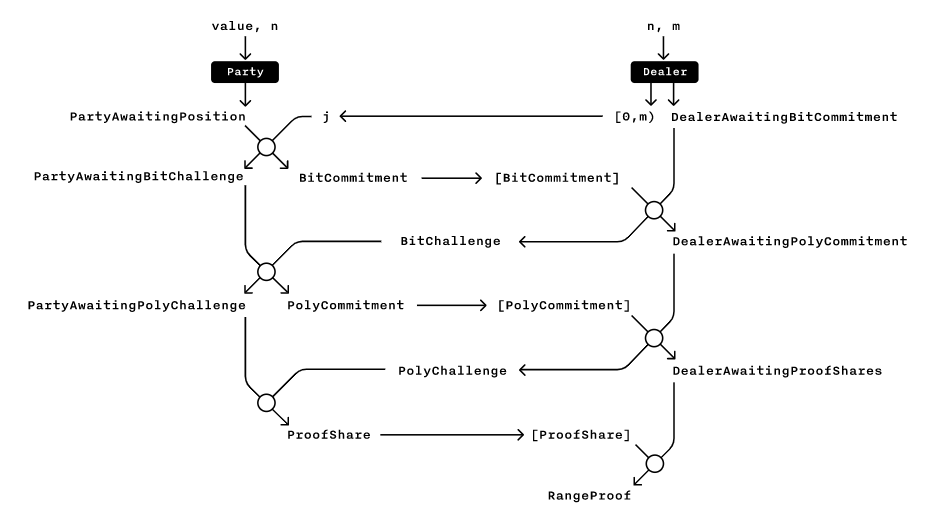
\includegraphics[scale=0.4]{img/multi-party protocol.png}
	\caption{
		Graph over type and function interactions. Graph from
		\cite{dalek-notes}.
	}
	\label{implementation-graph}
\end{figure}

This flow graph is an outline for the full Bulletproofs protocol, 
with each node being a function called in the code. Below we outline
a simplified pseudocode representing our implementation of this graph:

\begin{algorithm}[H]
	\DontPrintSemicolon
	\SetAlgoLined
	\KwIn{$n \in \Z, \vec{v}\in \Z^n_p, \vec{\bv} \in \Z^n_p, B\in\G, \bB\in\G, \vec{G}\in\G^n, \vec{H} \in\G^n$}
	\SetKwFunction{len}{.len()}
	\SetKwFunction{performChecks}{perform\_checks()}
	\SetKwFunction{createDealer}{create\_dealer($B,\bB,\vec{G},\vec{H},n,m$)}
	\SetKwFunction{createParty}{create\_Party($B,\bB,\vec{G},\vec{H},v,\bv,n$)}
	\SetKwFunction{computeAS}{create\_bit\_commitment($party\_step1, j$)}
	\SetKwFunction{firstaggregate}{receive\_bit\_commitments($dealer\_step1, \vec{V}, \vec{A},\vec{S}$)}
	\SetKwFunction{computeTs}{create\_poly\_commitment($party_j\_step2, \ran{y},\ran{z}$)}
	\SetKwFunction{secondaggregate}{receive\_poly\_commitments($dealer\_step2, \vec{T_1}, \vec{T_2}$)}
	\SetKwFunction{computetxB}{create\_proofshare($party_j\_step3,\ran{x}$)}
	\SetKwFunction{thirdaggregate}{receive\_proofshares($dealer\_step3,\vec{t(\ran{x})B}, \vec{\vec{\tt(\ran{x})\bB}}$)}
	$\performChecks$\\
	$m := \vec{v}\len$\\
	\tcp{DealerAwaitingBitCommitment}
	$dealer\_step1 := \createDealer$ \\
	\For{$j \in [1 : m+1]$}{
		\tcp{PartyAwaitingPosition}
		$party_j\_step1, V_j := \createParty$\\
		\tcp{PartyAwaitingBitChallenge}
		$party_j\_step2, A_j, S_j := \computeAS$
	}
	\tcp{DealerAwaitingPolyCommitment}
	$(dealer\_step2, \ran{y},\ran{z}) := \firstaggregate$\\

	\For{$j \in [1 : m+1]$}{
		\tcp{PartyAwaitingPolyChallenge}
		$(party_j\_step3, T_{1,j}, T_{2,j}) := \computeTs$
	}
	\tcp{DealerAwaitingProofShare}
	$(dealer\_step3, \ran{x}) := \secondaggregate$\\

	\For{$j\in [1 : m+1]$}{
		\tcp{ProofShare}
		$t(\ran{x})_jB, \tt (\ran{x})_j\bB := \computetxB$ 
	}
	\tcp{RangeProof}
	$aggregated\_rangeproof := \thirdaggregate$

	\Return{$(\vec{V}, aggregated\_rangeproof)$}

	\caption{Bulletproof algorithm}
\end{algorithm}

The functions called on lines 4, 12, 18, and 24 are from the
\texttt{dealer} module while the functions called on lines 7, 9, 15
and 21 are from the \texttt{party} module. Both sets of functions
correspond to the nodes in figure \ref{implementation-graph}
with the left nodes being the \texttt{party} functions and the right
nodes being the \texttt{dealer} functions. Each of these methods, in
the simplest terms, compute the values needed for the current step of 
the protocol, and generate the next party or dealer instance in the 
sequence. The names of these have been shortened due to formatting, 
but they correspond to types from figure \ref{implementation-graph}, 
with the graph names written as comments above the line where they 
are created in the pseudocode. 

The code we test against uses structs to represent the values for each 
of the different types of party and dealer, created by the methods 
described above. Each dealer struct implements the next function 
required to progress to the next \texttt{dealer} struct to make, and 
the same goes for each \texttt{party} struct. This way of implementing 
the methods ensures that a potential user of the crate cannot 
accidentally perform the steps out of order, due to the next step being 
integrated in the struct provided by the previous step.

When we began our implementation we made use of tuples to represent our
types instead, however, not using structs eventually caused severe 
code-bloating since tuples do not implement the \texttt{Copy} trait or 
\texttt{Clone} trait requiring some cumbersome and sizable rewrites. 
Not using structs also breaks the property of only being able to perform 
the steps in the right order, as outlined in figure \ref{implementation-graph}. 
Therefore, we switched to using structs which can derive the \texttt{clone} 
method automatically. 

There is however one place where our implementation differs from this 
convention. Namely with the \texttt{ProofShare} type. This is due to 
both the \texttt{dealer} and \texttt{party} modules needing direct access to the struct's 
definition, and due to the modular structure of our implementation, this 
was not possible as \texttt{ProofShare} instances created in the \texttt{party} 
module will have type \texttt{party::types::ProofShare} where the needed 
type is \texttt{types::ProofShare}. As such \texttt{ProofShare} is a 
simple type-alias tuple. This \textit{does} break the guarantee that the 
steps will always be performed in the right order, but this is not a major 
issue as our implementation is not meant to be used as a library, it is 
only intended for proving properties using proof assistants.

A big roadblock we hit while implementing this protocol was the
immense length it would have. This meant that writing any sort of test
for the code would require it to be finished in nearly its entirety.
This resulted in a lot of debugging through printing out values and manually comparing
them with the Dalek implementation. Another issue was the fact that
their library has built-in randomness. This meant that our code had
no way of utilizing the exact same random values, something that is
vital when comparing the implementations. Therefore, we forked their library and refactored
all their random values to be function inputs. This in no way
changes the functionality of the Dalek implementation, while allowing us to control the random values it uses, which we can then
match to our own, and thus allowing us to test against it.

Additionally, due to the lack of optimizations our implementation is
immensely slow, to the point where testing our full implementation
takes 22 hours to complete, while the equivalent checks for the Dalek
implementation takes a mere 2 minutes. To remedy this we instead
utilized a wrapper module to use the Dalek Ristretto implementation
instead of our own, as was done when testing the inner product proof
(section \ref{implementing-inner-product-proof}). This significantly
increased the speed of our implementation and thus allowed much more
rigorous testing.

To keep our implementation as simple as possible we only implemented
what would be equivalent to the \texttt{prove\_multiple\_with\_rng()}
method from the crate we test against. We felt this was sufficient as
the \texttt{prove\_multiple()}, \texttt{prove\_single\_with\_rng()}
and \texttt{prove\_single} methods would all call
\texttt{prove\_multiple\_with\_rng()} in some way. Thus, the 
implementation of these functions seem too trivial to implement.

\textbf{Testing:}

To test the code we created a main helper function \texttt{fn
test\_bulletproofs(m:usize, n:usize)}:

\begin{lstlisting}
fn test_bulletproofs(m: usize, n: usize) {
	let (bp_gens_hac, bp_gens_rust) = create_bp_gens(number_of_values, n);
	let (pc_gens_hac, pc_gens_rust) = create_pc_gens();
	let (transcript_hac, mut transcript_rust) = create_transcript();

	let (values_hac, values_rust) = generate_random_values(number_of_values, n);
	let (blindings_hac, blindings_rust) = generate_random_scalars(number_of_values);
	let (a_blindings_hac, a_blindings_rust) = generate_random_scalars(number_of_values);
	let (s_blindings_hac, s_blindings_rust) = generate_random_scalars(number_of_values);
	let (s_L_hac, s_L_rust) = generate_many_random_scalars(n, number_of_values);
	let (s_R_hac, s_R_rust) = generate_many_random_scalars(n, number_of_values);
	let (t1_blindings_hac, t1_blindings_rust) = generate_random_scalars(number_of_values);
	let (t2_blindings_hac, t2_blindings_rust) = generate_random_scalars(number_of_values);
\end{lstlisting}

\texttt{BulletproofGens} and \texttt{PedersenGens} are converted from
the Dalek implementation and the transcripts are initialized
with the same label. The rest of the values, except \texttt{n} and
\texttt{m}, are generated randomly using helper functions. The values
\texttt{n} and \texttt{m} are taken as function parameters. This lets
us run many short test functions testing for different \texttt{m}'s
and \texttt{n}'s:

\begin{lstlisting}
#[test]
fn i2j8() {
    test_bulletproofs(2,8);
}

#[test]
fn i2j16() {
    test_bulletproofs(2,16);
}
...
\end{lstlisting}

After running a single test for most combinations of $n$ and $m$, to
test all modules in one test, we replaced the Hacspec Ristretto library
with our wrapped library which uses the Rust Ristretto crate. This greatly increased speed and therefore
the amount of tests we were able to run. Below is a table of what tests 
were done and how long they took:

\begin{center}
\begin{tabular}{ c|c|c|c } 
	& Using Hacspec Ristretto & Using Dalek Ristretto & Times faster\\ \hline\hline
	$n = 8, m = 2$    & 420.02 s     & 0.57  & 736.84 \\ \hline 
	$n = 16, m = 2$   & 809.14 s     & 0.97  & 834.16 \\ \hline 
	$n = 32, m = 2$   & 1,563.87 s   & 1.83  & 854.57 \\ \hline 
	$n = 64, m = 2$   & 2,073.97 s   & 3.56  & 582.57 \\ \hline 
	\hline\hline
	$n = 8, m = 4$    & 823.68 s     & 0.97  & 849.15 \\ \hline 
	$n = 16, m = 4$   & 1,585.96 s   & 1.79  & 886.01 \\ \hline 
	$n = 32, m = 4$   & 3,075.16 s   & 3.32  & 926.25 \\ \hline 
	$n = 64, m = 4$   & 6,107.19 s   & 6.55  & 932.39 \\ \hline 
	\hline\hline
	$n = 8, m = 8$    & 1,624.98 s   & 1.85  & 878.36 \\ \hline 
	$n = 16, m = 8$   & 3,127.60 s   & 3.49  & 896.16 \\ \hline 
	$n = 32, m = 8$   & 6,114.07 s   & 6.63  & 922.18 \\ \hline 
	$n = 64, m = 8$   & 10,418.94 s  & 12.69 & 821.03 \\ \hline 
	\hline\hline
	$n = 8, m = 16$   & 3,191.85 s   & 3.63  & 879.29 \\ \hline 
	$n = 16, m = 16$  & 6,209.07 s   & 7.20  & 862.37 \\ \hline 
	$n = 32, m = 16$  & 12,246.25 s  & 13.56 & 903.11 \\ \hline 
	$n = 64, m = 16$  & 24,303.13 s  & 26.06 & 932.58 \\ \hline 
	\hline\hline
	$n = 64, m = 32$  & 39,100.84 s  & 41.70 & 937.67 \\ \hline 
	\hline\hline
	$n = 64, m = 64$  & 67,508.52 s  & 64.59 & 1,045.18 \\ \hline 
\end{tabular}
\end{center}

With these performance increases we ran 5,000 tests on randomized
$n$ and $m$ values, which all successfully passed, taking 43,017.28
seconds. The reason we did not run more tests is because, despite these
speed increases, it still runs slow compared to other libraries. This
means that the Bulletproofs library is not as thoroughly tested,
which does make the property of equivalence between the Bulletproof
implementations weaker compared to the other libraries. This is mediated
by how comprehensive the protocol is, meaning a single randomized
test passing is good evidence to support that the code functions properly for
that combination of $n$ and $m$. With 5,000 tests we have 200 tests
for each combination of inputs on average.

\section{Future work:} \label{future-work}

Currently, our implementation functions as intended, however parts has
yet to be properly merged into Hacspec. This is still being worked on in
collaboration with the Hacspec team. This process can take time and will
involve refactoring parts of the code to improve overall code quality.

After this is completed the intended work is finished, but the obvious
next step is to use a proof assistant on our implementations to
prove properties about the equivalent, but much faster, Rust
implementations. This would reduce the risk of vulnerabilities in the
Rust implementations.

More thorough testing could be done to ensure that the Hacspec and
Rust implementations function identically, which could involve writing
more property-based and unit tests as well as running tests longer.

\section{Conclusion:} \label{conclusions}

Our intended goal of a complete implementation of Bulletproofs was
achieved. Necessary modules, namely Ristretto and Merlin were also
implemented. These implementations are constructed in a way that
makes them function identically to their Rust counterparts, with high
probability, due to rigorous property-based testing. Thus, by proving
properties about our implementation, those same properties should hold
for the respective Rust implementations.

Additionally, we have also highlighted how a somewhat abstract
cryptographic protocol could be implemented in Hacspec. Thus, it can
act as a reference for how such protocols might be implemented and
an example of how to utilize our Ristretto and Merlin modules.

In essence, we have laid nearly all the groundwork for the future work
of proving properties about the Rust implementations, and introduced a
few powerful building blocks allowing future developers to more easily
implement other cryptographic algorithms, by allowing them to use our
Ristretto25519 and Merlin modules for implementing protocols applying
elliptic-curve cryptography and zero-knowledge proofs respectively.

\section{References} \label{references}
\printbibliography

\end{document}
